\documentclass[10pt, a4paper, openany]{book}
\usepackage{../generalStyle}

\begin{document}

\title{Programmazione Dispositivi Mobili}

\author{Sara Angeretti}

\date{2024/2025}

\maketitle

\tableofcontents

% 01/10/2025

\chapter{Introduzione al corso}
\section{Organizzazione}
\par In più rispetto all'ultimo semestre:
\begin{itemize}
    \item "gettoni presenza" per punti bonus
    \item 15 ottobre: conferenza azienda (BendingSpoons) su iOs
\end{itemize}

\section{Obiettivi del corso}
\par Il corso ha come obiettivo acquisire:
\begin{itemize}
    \item \textbf{\underline{Conoscenze}} (principi di buona programmazione) relative al mondo dello sviluppo mobile
    \item \textbf{\underline{Competenze}} sullo sviluppo Android 
\end{itemize}
\par Ma perché è stato scelto proprio Android? Comporta diversi vantaggi rispetto ad altri sistemi operativi come iOs:
\begin{itemize}
    \item più open source
    \item essendo più open source conosciuto meglio dai docenti che sono quindi più in grado di insegnare e correggere
    \item Android, nel caso uno voglia poi accedere allo Store e pubblicare un'app, prevede una tassa di iscrizione di \texttildelow 25\$ \textbf{una tantum}, mentre per iOs è di 100\$ ma penso sia \textit{annuale}.
\end{itemize}
\par Alla fine del corso dovremo essere in grado di:
\begin{itemize}
    \item Sviluppare un'applicazione ``from scratch'' che segua l'\textbf{\underline{architettura}} di riferimento Android
    \begin{itemize}
        \item alla fine se abbiamo rispettato o no l'architettura presentata a lezione è quello che guardano di più della nostra app, se non è bellissima o funzionante al 101\% importa meno
    \end{itemize}
    \item Comprendere il funzionamento di applicazioni Android
\end{itemize} 

\section{Il corso in pillole}
\begin{enumerate}
    \item \textbf{Introduzione} alla progettazione e allo sviluppo di applicazioni mobili
    \item \textbf{Linee guida} sull'architettura dell'app
    \item \textbf{Sviluppo} di un'app in Java\\
    Per il nostro progetto possiamo usare Java o Kotlin, la teoria rimane la stessa, ma a lezione useremo solo Java. Questo perché è già stato presentato ed usato in altri due corsi e quindi conosciuto meglio da docenti e studenti. Inoltre, è previsto (penso in entrambi i linguaggi) l'uso di lambda functions, più elegante e funzionale in Kotlin, però buono anche in Java. Infine, Java risulta più conveniente per l'uso di librerie esterne di Kotlin, che è più giovane e meno conosciuto e quindi ha meno librerie disponibili.\\
    Eventualmente, sul sito Google ci sono disponibili diversi tutorial gratuiti (video) per imparare Kotlin e per la migrazione del mio progetto da Kotlin a Java.\\
    Se si vuole utilizzare Kotlin, c'è da scrivere alla professoressa spiegando le ragioni della scelta.\\
    L'app deve essere robusta. La robustezza si basa sull'autonomia dalla connessione di rete. Il concetto ``\underline{offline-first}'' è molto importante, prima di tutto l'app deve funzionare senza connessione. Inoltre, deve essere anche \underline{evolvibile}. Oltre ai suoi componenti funzionali (ovvero le sue \underline{funzionalità}) di base, ci sono determinate funzionalità che devono essere mantenute ed evolute/ampliate nel tempo.\\
    La nostra app deve essere:
    \begin{enumerate}
        \item Compliant con l'architettura di riferimento\\
        La cosa \underline{importante} della nostra app non è l'estetica o se funziona bene, ma \textbf{\underline{come}} l'architettura presentata a lezione viene sviluppata.
        \item Con UI
        \item Che accede alla rete per i dati (API esterne)
        \item Che fa persistenza (\underline{locale + remoto})\\
        Ovvero deve funzionare \textit{localmente} e salvare localmente i dati (importante per il concetto di ``\textit{offline-first}''). Però deve anche salvare \textit{in remoto} i dati, ma deve rispettare la \textit{cross-device synchronization}.\\
        Importante per quanto riguarda la \underline{cross-device synchronization}, ovvero deve funzionare su diversi dispositivi con stato sincronizzato.
        \item Che usa Firebase\\
        Firebase è un framework di Google che offre una serie di servizi per lo sviluppo di applicazioni mobili.
    \end{enumerate}
\end{enumerate}

\section{Il progetto}
\begin{itemize}
    \item Durante il corso si porta avanti un progetto che sarà oggetto dell'esame finale
    \item Il progetto è svolto in maniera paritaria da un gruppo di studenti
    \begin{itemize}
        \item Composto da almeno 3 persone e fino ad un massimo di 5
        \item Eccezioni verranno valutate singolarmente
    \end{itemize}
    \item Il progetto è proposto dal gruppo (scadenza 17 ottobre 2025)
    \begin{itemize}
        \item L'idea può anche essere non nuova, ad esempio un'app che mostra i film e le recensioni\dots
    \end{itemize}
    \item Il progetto deve essere sviluppato per Android (in Java)
    \item \underline{Assistenza al progetto} (oltre che ai laboratori durante i quali lavoreremo sul \textbf{nostro} progetto) verrà fornita \textit{eventualmente} anche durante le \underline{esercitazioni} (durante le quali vedremo come realizzare un'applicazione da zero tramite un \textit{progetto} \underline{scelto dal docente} con le proprie funzionalità e sviluppato \textbf{\underline{esattamente}} come vuole la prof che sia realizzata la nostra app)
    \item Si suggerisce caldamente per chi voglia sfruttare l'appello invernale per sostenere l'esame di seguire i laboratori perché verrà fornita assistenza.
    \item L'app deve \textbf{NECESSARIAMENTE} avere:
    \begin{enumerate}
        \item architettura
        \item almeno 1 API esterna
        \item autenticazione se necessario
        \item off-line first (deve funzionare fluidamente anche in assenza di connettività)
        \item cross-device synchronization
        \item testing
        \item layout grafico (importante ma meno del resto)
        \item storage locale (opzionale: se necessario, ma ne va giustificata l'assenza in caso)
        \item documentazione di buona qualità (ci sono molti esempi sul drive presente su Moodle)
    \end{enumerate}
    \item Bisogna usare GitLab o GitHub (non per forza ma una settimana prima della consegna va fatto quindi tanto vale)
\end{itemize}

\subsubsection{Valutazione}
\begin{itemize}
    \item Codice sorgente e documentazione della nostra app con dentro:
    \begin{enumerate}
        \item Scelte architetturali
        \item Uso di API esterne (in maniera sensata)
        \item Uso storage locale, per offline-first
        \item Uso del framework Firebase (autenticazione), per cross-device synchronization
        \item Layout grafico che sia (circa) sensato, per es. tramite uso librerie di material design
        \item Documentazione
    \end{enumerate}
    \item Punti 1-5 chiaramente via Software, 6 cartaceo
    \item Uso di GitLab o GitHub (da aggiungere account fornito dai docenti)
\end{itemize}

\subsection{1. Scelte architetturali}
\begin{center}
    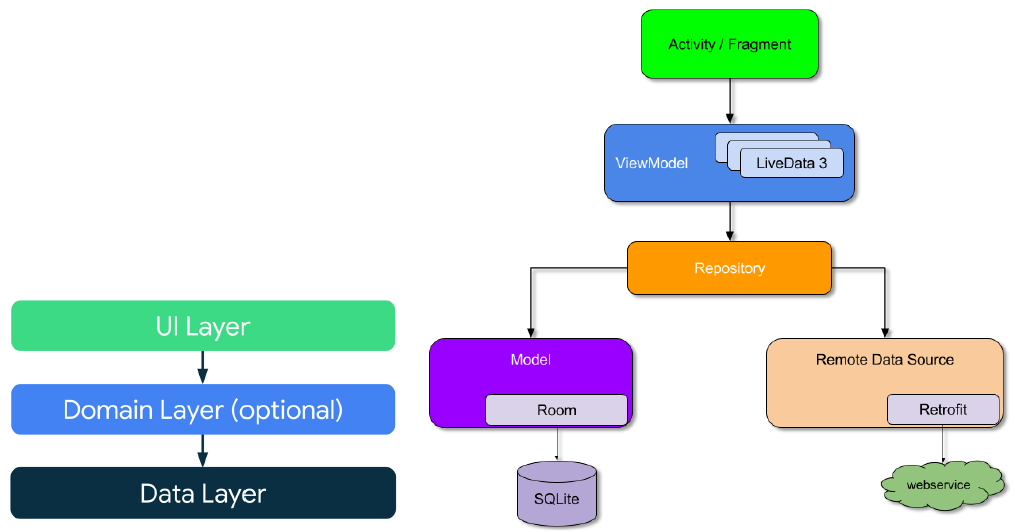
\includegraphics[width=0.5\textwidth]{images/00_scelte_architetturali1.png}
\end{center}
\par Queste 5 entità \textbf{\underline{devono}} essere presenti nel nostro progetto.

\subsection{2. Uso di API esterne}
\par Esempi di API esterne (gratuite):
\begin{itemize}
    \item Immagini
    \begin{itemize}
        \item \url{https://unsplash.com/developers}
        \item \url{https://developers.google.com/maps/documentation/places/web-service/photos}
    \end{itemize}
    \item Video Giochi
    \begin{itemize}
        \item \url{https://www.igdb.com/api}
    \end{itemize}
    \item Film
    \begin{itemize}
        \item Film
        \item MovieDB
        \item Open Moview DB
        \item IMDb
        \item The Moview DB
    \end{itemize}
    \item Qualità dell'aria
    \begin{itemize}
        \item \url{https://aqicn.org/}
    \end{itemize}
    \item Cibo
    \begin{itemize}
        \item TheMealDB.com
        \item \url{https://spoonacular.com/food-api}
    \end{itemize}
    \item Meteo
    \begin{itemize}
        \item \url{https://openweathermap.org/current}
    \end{itemize}
    \item …
\end{itemize}
\par Tante disponibili free
\begin{itemize}
    \item \url{https://github.com/public-apis/public-apis}
\end{itemize}
\par Postman è un'applicazione che permette di testare le API, di interrogarle, è molto utile per vedere come funzionano le API e come si comportano prima di integrarle. \url{https://www.postman.com/}

\subsection{3. 4. 5. Uso di Firebase}
\par Strumento molto potente, lo vedremo ad esercitazione. Ti aiuta a creare:
\begin{itemize}
    \item Autenticazione
    \begin{itemize}
        \item se necessario nell'app
    \end{itemize}
    \item Database remoto
    \begin{itemize}
        \item Anche a supporto della cross-device synchronization
    \end{itemize}
    \item Notifiche push
    \item \dots
\end{itemize}

\subsection{6. Testing}
\begin{itemize}
    \item JUnit 4/5
    \item Mockito/MockK
    \item Espresso (per test UI, con un input di testo e comandi per interagire con l'UI) !!!
    \item Robolectric
    \item Firebase Test lab
    \item UI Automator (quella che mi permette di fare il cross-app testing) !!!
\end{itemize}
Quelli con "!!!" sono quelli evidenziati dalla prof.

\subsection{7. Layout grafico}
\par Non una delle cose essenziali ma comunque importante, l'app deve comunque essere user-friendly.
\par Ho delle regole da seguire, il progetto deve seguire i principi di material design (che sono linee guida di Google per lo sviluppo di UI, ma ci sono anche widget grafici, gratuiti ed usabili). Per esempio: color extraction (tutti i widget hanno colorazione uniformata allo sfondo per conferire maggiore fluidità).
\begin{center}
    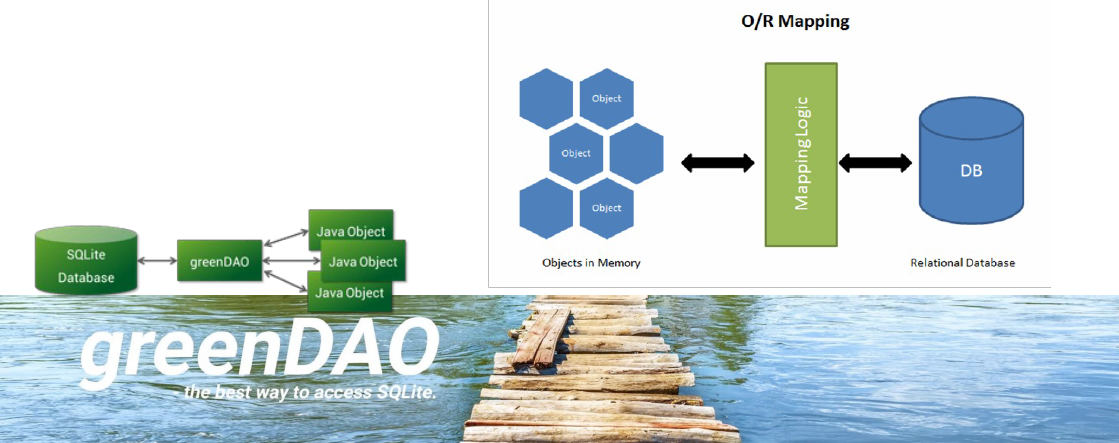
\includegraphics[width=0.5\textwidth]{images/00_orm1.png}
\end{center}

\subsection{8. Uso ORM - Object Relational Mapping}
\par Uso di ORM (Object-relational mapping). Due tool sono:
\begin{itemize}
    \item Room (integrato in Android), utile per persistenza
    \item greenDao, più vecchio ma ancora in uso
\end{itemize}

\subsection{Documentazione}
\par La documentazione dovrà essere strutturata in 3 sezioni:
\begin{enumerate}
    \item le \textbf{funzionalità offerte}
    \begin{itemize}
        \item potete scriverle in italiano, oppure usare degli use case
    \end{itemize}
    \item l'\textbf{architettura complessiva} che specifica i componenti da voi sviluppati e le loro relazioni e modalità di comunicazione con eventuali componenti esterni utilizzati
    \begin{itemize}
        \item Firebase, API esterne, DB interno, etc.
    \end{itemize}
    \item il \textbf{design della soluzione} che include i \textit{componenti} che avete sviluppato (inteso come Fragment, Activity, etc.), le loro \textit{responsabilità} (cioè cosa fanno) le loro \textit{modalità di interazione}
\end{enumerate}
\par Alcuni esempi, sul drive fornito dalla prof su Moodle.

% \subsection{Discussione progetto}
% \begin{itemize}
%     \item 24 gennaio 2025, \texttildelow 09:00
%     \item 21 febbraio 2025, \texttildelow 09:00
% \end{itemize}

\subsection{Scadenze}
\begin{itemize}
    \item \underline{10 ottobre 2025}: comunicazione gruppo
    \begin{itemize}
        \item la composizione del gruppo (matricola, cognome, nome), un nominativo per riga;
        \item il referente del gruppo.
    \end{itemize}
    \item \underline{17 ottobre 2025}: comunicazione argomento progetto
    \begin{itemize}
        \item Il titolo del progetto;
        \item una descrizione del progetto che si intende svolgere;
        \item il referente del gruppo.
    \end{itemize}
\end{itemize}


% 03/10/2024

% \chapter{Introduzione ai dispositivi mobili}
% 09/10/2024

\chapter{Costo Sviluppo Mobile}
\par Diversi fattori influenzano il costo di sviluppo di un'applicazione mobile, tra cui:
\begin{itemize}
    \item piattaforma target
    \item caratteristiche
    \item design
    \item eventuale infrastruttura aggiuntiva 
    \item il team di sviluppo (non per forza uno unico per diverse piattaforme, es. uno per Android, uno per iOs)
\end{itemize}

\subsection{Fattore \#1: Piattaforma Target}
\par La scelta della piattaforma target è uno dei fattori più importanti che influenzano il costo di sviluppo di un'applicazione mobile. Più piattaforme saranno supportate e più alto sarà il costo. Devo aver ben presente a quale mercato voglio indirizzare il mio prodotto.
\par Fortunatamente, non è sempre proporzionale al numero di piattaforme supportate, grazie al \textbf{riutilizzo del codice}. 
\par Prima si realizza su una piattaforma e, una volta creata l'architettura (che vado ad implementare per la mia piattaforma) e validata l'idea, si può replicare su altre piattaforme.

\subsection{Fattore \#2: Obiettivi e modello di sviluppo}
\par Determinare gli \textbf{obiettivi di business} e quindi \textit{cosa} dovrà fare l'app, gli obiettivi che deve raggiungere. Es.: tutto ciò che un utente vuole fare senza essere obbligato a stare bloccato davanti ad un computer, un browser. Es.: l'app di una banca.
\par Se sbaglio, butto via un sacco di soldi. Per questo è legato ai costi.
\par \`E necessario creare un \textbf{documento di specifiche tecniche} che elenchi le caratteristiche che l'app avrà.
\par Devo decidere il modello di sviluppo:
\begin{itemize}
    \item Set fisso di caratteristiche
    \item Set dinamico di caratteristiche
    \item Mix: si inizia con una serie di requisiti fissi, ma i clienti hanno una certa flessibilità nel poter decidere di cambiare qualcosa
\end{itemize}
\par Chiaramente il meglio è l'ultimo perché si ha una certa flessibilità, se facessi un set più fisso rischierei di non soddisfare le esigenze del cliente e dover buttare via tutto e quindi aumentare i costi. Ci serve un approccio ``\textit{agile}'', ovvero un approccio che permetta di cambiare le cose in corso d'opera. Vado avanti a pochi obiettivi alla volta (\textit{``user stories''}, per dire l'autenticazione, creazione di un bonifico, vedere i movimenti, sono tutti esempi di user stories), con un ciclo di sviluppo molto breve, e poi passo al prossimo obiettivo. Facendo poco alla volta posso affrontare i miei \textit{debiti tecnologici} (ciò che devo studiarmi man mano perché non conosco) e sentirmi con gli \textit{stackholder} (chi ha interesse nel progetto) per capire se sto andando nella direzione giusta.

\subsection{Fattore \#3: Design}
\par Il design delle app (\underline{sia UI} (come sono i bottoni, i tasti\dots) \underline{che UX} (come l'utente riesce a navigare, a sfruttare le capacità dell'app)) è ciò che separa le buone app da quelle \textit{amazing}.
\begin{itemize}
    \item \textbf{Design classico:} con cui gli utenti hanno più familiarità, meno costoso (es. il design classico di Apple per le applicazioni iOS)
    \item \textbf{Design impressive:} più costoso, richiede più tempo e risorse, ma può fare la differenza
\end{itemize}

\subsection{UI \& UX}
% Slide, titolo rosa perché è un'aggiunta optional, non è fondamentale
\par Diversi ruoli, diverse skills e competenze. Ha nominato Figma che aiuta a "disegnare/creare" i prototipi delle app.

\subsection{Fattore \#4: Come Sviluppare?}
\par Che strumenti uso? Anche questa scelta incide sui costi. C'è nelle slide una lista di \underline{piattaforme di sviluppo di applicazioni mobili}, di \underline{strumenti cross-platform} e di \underline{sviluppo nativo}.
\par Ha nominato \textbf{Flutter} come strumento cross-platform, che permette di scrivere una volta sola il codice e poi eseguirlo su diverse piattaforme. \`E la cosa più vicina a sviluppo nativo però (se ho capito bene).

\subsection{Fattore \#5: Caratteristiche dell'app}
\par Le caratteristiche dell'app sono il fattore determinante per il costo dell'app stessa. Con l'aumentare del numero e della complessità delle funzioni della app, aumenta anche il costo di sviluppo.
\par Es.: è una to-do list app? Poche semplici funzionalità. Include mail e autenticazione? Richiede l'uso del GPS? Già diverso. Etc.

\subsection{Fattore \#6: Infrastrutture}
\par Un'app che si appoggia ad un componente remoto ha costi di sviluppo più alti di una "off-line".
\par \`E necessario prendere in considerazione, tra le altre cose:
\begin{itemize}
    \item configurazione del server
    \item requisiti di memorizzazione 
    \item crittografia e sicurezza dei dati
    \item comunicazione con l'app
    \item gestione degli utenti
    \item \dots
\end{itemize}

\subsection{Fattore \#7: Altri costi oltre a quelli di sviluppo}
\par Oltre ai costi di sviluppo, ci sono altri costi da considerare:
\begin{itemize}
    \item \textbf{Account dello sviluppatore (Developer Account):} c'è la slide
    \item \textbf{Componenti server-side e servizi Cloud:} c'è la slide
    \item \textbf{Manutenzione dell'app}:
    \begin{itemize}
        \item Molte app zombie
        \item Se non si vuole - guarda la slide
    \end{itemize}
\end{itemize}
\par Grafico di proiezione del guadagno da app: è in crescita, questo anche perché (come ha mostrato uno studio) un utente tende a preferire un'applicazione ad un sito web. Perciò se ho sia un'app che una web app che svolgono gli stessi compiti, l'utente tenderà a preferire l'applicazione.

\subsubsection{*: App zombie}
\par Sono app non gestite. Avevamo parlato di una curva grafico che mostrava quante app sono state eliminate dall'Android App Store, questo era successo anche per la gran quantità di app non gestite o mantenute nel tempo che sono state tirate giù.

\section{Monetizzazione}
\par \textbf{Monetizzare un'app significa implementare strategie che permettano di generare, al proprietario dell'app, entrate attraverso il suo utlizzzo}. Slide

\subsection{Purchase-app-once (paid app)}
\par Quasi 95\% delle app sono gratuite. Tuttavia ci sono utenti che \textbf{pagheranno} per applicazioni di \textbf{qualità} che soddisfino un bisogno molto specifico, da pochi centesimi a centinaia di euro.

\subsection{Freemium app}
\par Prevede due o più varianti del prodotto da distribuire a prezzi diversi. Di solito due varianti:
\begin{itemize}
    \item \textbf{Versione Base:} gratuita
    \item \textbf{Versione Premium:} a pagamento, include funzioni e/o contenuti aggiuntivi (es.: sblocco livelli) o rimuove pubblicità
\end{itemize}
\par Filosofia: dare un

\subsection{Subscription app}
\par Gli utenti \textbf{pagano un canone} periodico per l'utilizzo della app. Funziona bene per app che:
\begin{itemize}
    \item si basano su un \textit{servizio di backend}
    \item forniscono l'\textit{accesso a contenuti aggiornati costantemente}
\end{itemize}
\par Gli utenti, pagando un canone, si aspettano di ricevere più di quanto offra una paid app. Le app in abbonamento devono fornire continuamente nuovi contenuti e/o funzioni.

\subsection{In-app purchases}
% 10/10/2024

\chapter{Esercitazione 1}
\section{Passi su Android Studio}
\begin{itemize}
    \item New Project
    \item Empty Views Activity
    \item Scegliamo linguaggio Java
\end{itemize}
\par Da terminale (seconda icona dal basso a sinistra) possiamo scrivere:
\begin{enumerate}
    \item \texttt{git init} per inizializzare una repository (fatta dentro perché ci lavoro dentro Android Studio e non da VSCode come faccio con tutte le altre repository)
    \item \texttt{levels} per vedere i livelli di git
    \begin{itemize}
        \item da prompt dei comandi \texttt{dir} per vedere la lista di directory e file, ma forse è un livello solo, NON LO SO CONTROLLA. \texttt{dir} su Windows, \texttt{ls -a} su Linux.
    \end{itemize}
    \item \texttt{git commit} per fare un commit
    \item \texttt{git branch nomebranch} per creare un nuovo branch
    \item \texttt{git checkout -b nomebranch} ne crea uno nuovo
    \item \texttt{git checkout} si aspetta il nome del branch
    \item \texttt{git checkout nomebranch1} per passare al branch nomebranch1
    \item \texttt{git checkout nomebranch2} per passare al branch nomebranch2\\
    Se faccio commit su modifiche non pushate, rischio di andare incontro a conflitti.\\
    L'asterisco (sul sito \url{https://learngitbranching.js.org/}) mi indica su quale branch mi trovo.
    \item \texttt{git merge nomebranch} per fare il merge in nomebranch del branch in cui mi trovo (quello attivo in quello più stabile)
    \item \texttt{git rebase nomebranch} per fare il rebase in nomebranch del branch in cui mi trovo: è un'alternativa a merge, "riscrive la storia", collassa tutti i branch in uno cancellando la storia di quello in cui mi trovo e mettendola in quello in cui voglio fare il rebase.
    \item \texttt{git revert nomedelcommit} per fare il revert di un commit, tornare al commit (es. c6) e cancellare le modifiche da quel commit in poi, magari per eliminare branch che ho fatto inutilmente.
\end{enumerate}
\par GitHub sul suo sito ha una sezione (\url{https://docs.github.com/en}) con una serie di guide su come usare git.

\subsection{Sito per simulare funzionamento di git}
\url{https://learngitbranching.js.org/}

\subsection{Comandi git da terminale}
\par Le commit, partendo dalla cartella del progetto:
\begin{itemize}
    \item \texttt{git pull}
    \item \texttt{git add .}: mette tutto ciò che c'è nella working area nella staging area, il punto mi dice "tutti i file"
    \item \texttt{git commit -m "messaggio in cui dico cosa ho fatto in breve"}: mette tutto ciò che c'è nella staging area nella commit area
    \item \texttt{git push}
\end{itemize}

\subsection{I conflitti}
\par In caso di conflitti, per arrivare alla pagina di risoluzione dei conflitti (al centro versione locale, a sinistra un branch e a destra l'altro), quando si verifica un conflitto esce un pulsante "risolvi conflitti" magari in inglese. Tendenzialmente il main è la versione più stabile, quindi si fa il merge del branch in cui si è lavorato in main.
\par Consiglia di fare branch per funzionalità e non per persona, però è un approccio personale e comunque l'importante è essere consistenti.


\par Git Ignore è un file che va ad appuntare estensioni di file o file o cartelle da ignorare. Al momento dell'inizializzazione del progetto avremo già una lista di file di base ignorati. Di solito i file compilati (es su Java i \texttt{.class}) sono da ignorare.
\par Il sito \url{gitignore.io} permette di generare un file \texttt{.gitignore} in base al linguaggio di programmazione che si sta utilizzando con i file da ignorare. Metto Android, Windows. Consiglia di farlo all'inizio anche per alleggerire la compilazione.

\par GitHub e GitLab sono istanze di git, mentre git è il programma generico.

\subsection{Il progetto}
\par Prima cosa da fare: avviare la repository, il gitignore, il README. Decidere come gestire i branch (non valutato, ma l'approccio deve essere consistente) se per team o funzionalità o cosa, vedi online. Dice che ci dovrebbero essere consigli. Meglio tenere il main branch come quello che funziona di più.
\par Per creare una nuova repository su GitHub:
\begin{itemize}
    \item scelgo nome e descrizione
    \item scelgo se pubblica o privata (per il progetto può anche essere privata perché tanto posso aggiungere dopo chi può accedervi)
    \item posso scegliere se aggiungere un README (che è un file markdown che appare nella home della repository) e un \texttt{.gitignore} (che posso scegliere in base al linguaggio di programmazione che sto usando), ma sono cose che posso aggiungere anche dopo
    \item posso scegliere se installare la repository tramite set up desktop, da linea di comando (sono i comandi che abbiamo visto prima) o pushare da linea di comando una repo già esistente
    \begin{itemize}
        \item l'unica riga che non abbiamo visto è \texttt{git remote add origin url}, che serve per collegare la repository locale a quella remota
    \end{itemize}
\end{itemize}
% 11/10/2024

\chapter{Tipi di applicazioni}
\section{Situazione ad oggi}
\par \textbf{Due principali player} (iOs e Android). Nonostante questo, gli sviluppatori hanno a disposizione:
\begin{itemize}
    \item molti linguaggi di programmazione
    \begin{itemize}
        \item Java
        \item Swift
        \item JavaScript
        \item Dart
        \item \dots
    \end{itemize}
    \item Molti framework
    \begin{itemize}
        \item Cordova
        \item React Native
        \item Xamarin
        \item Flutter
        \item \dots
    \end{itemize}
    \item E soprattutto, molte architetture
    \begin{itemize}
        \item app native (oggetto di questo corso)
        \item web app
        \item app ibride
        \item progressive web app
        \item app cross-compiled
    \end{itemize}
    Per scegliere la migliore, devo considerare l'oggetto del mio progetto (alcuni linguaggi/framework sono più adatti di altri), il tipo di applicazione che voglio realizzare, il tempo a disposizione, il budget, le competenze del team, \dots
\end{itemize}

\section{Livelli di astrazione}
\subsection{Livello più basso: hardware}
\par L'hardware Apple è proprio dell'azienda Apple, poi magari varia da modello a modello ma è sempre lo stesso costruttore.
\par L'hardware Android è invece prodotto da diversi costruttori, quindi varia molto da modello a modello.
\begin{itemize}
    \item es.: Google, Samsung, Huawei, Xiaomi, LG, Motorola\dots
\end{itemize}
\par Su questi hardware andiamo a implementare \textbf{app native} (così chiamate perché vanno ad usare il 100\% delle API messe a disposizione dal sistema operativo). I linguaggi nativi per implementare queste app sono:
\begin{itemize}
    \item Android
    \begin{itemize}
        \item Java (dal 2007 nel panorama Android)
        \begin{itemize}
            \item compiliamo per linguaggio intermedio (bytecode) e poi viene eseguito da una JVM (Java Virtual Machine); scrivo in un'unica codebase su cui compilo nel momento in cui viene eseguito e quindi sulla piattaforma effettiva
        \end{itemize}
        \item Kotlin (\texttildelow 2008????)
        \item Problema è che ogni volta che viene rilasciata una nuova API deve essere sviluppata sia in Java che in Kotlin.
        \item (NDK) la sigla significa \textit{Native Development Kit}, permette di scrivere codice in C/C++ e di interfacciarsi con il codice Java.
    \end{itemize}
    \item iOs
    \begin{itemize}
        \item Objective-C 
        \item Swift
        \begin{itemize}
            \item linguaggio di paradigma molto più moderno rispetto a Objective-C che nasce da C e quindi si porta dietro molte complicazioni
        \end{itemize}
    \end{itemize}
\end{itemize}

\subsection{App native}
\subsubsection{Caratteristiche}
Slide con lista
\begin{itemize}
    \item specifico s.o.
    \item codice binario scaricato e memorizzato nel file system
    \item app store o marketplace (anche Apple ha perso la causa ed è costretta a rendere le sue app disponibili anche su altri store/marketplace)
    \item eseguita direttamente dal s.o. 
    \begin{itemize}
        \item viene lanciata attraverso la schermata home del dispositivo con un ``tap'' (tocco l'icona e parte, non ci sono passaggi intermedi)
        \item non contiene un container app in cui girare (ho perso cos'ha detto a voce)
    \end{itemize}
    \item l'app fa uso diretto delle API del s.o. (GPS, fotocamera, accelerometro, \dots) (avevamo visto a prog2, Java mette a disposizione una SDK, una libreria, per facilitare la programmazione). Porgrammando da d.m. faremo un uso intenso delle API del sistema su cui mi trovo e ci dovremo interfacciare molto con l'hardware. Abbiamo:
    \begin{itemize}
        \item strato sotto: hardware
        \item strato intermedio: sistema operativo che si interfaccia con l'hardware da solo senza che ci debba pensare io
        \item strato sopra: API, che il s.o. mette a disposizione per interfacciarsi con l'hardware senza interfacciarsi con l'hardware
        \item strato ancora più sopra: SDK librerie che mi permettono di interfacciarmi con le API
        \item strato ancora più sopra: open SDK, quello che effettivamente andrò ad usare (es. \texttt{open file()}, \texttt{append()}, \dots)
    \end{itemize}
    Questo è il bello dello sviluppare nativo: lavorare con le API al 100\% e poter sfruttare al massimo le potenzialità del dispositivo
\end{itemize}

\subsubsection{Processo di generazione}
\par Abbiamo: 
\begin{center}
    \begin{tabular}{ |c c c c c| }
        \hline
        \textbf{Codice sorgente} (Java) & $\rightarrow$ & & $\rightarrow$ & Risorse (es. img) \\
        \hline
        \textbf{Compilatore} e \textbf{Linker} & $\rightarrow$ & Eseguibile (binario) & $\rightarrow$ & \textbf{Packager} \\
        \hline
        & & & & \textbf{Packager distribuibile} (\texttt{.apk}, \texttt{.apks}, \texttt{bundle}) \\
        \hline
        & & & & App store\\
        \hline
    \end{tabular}
\end{center}

\subsubsection{Interazione con il dispositivo}
\par Slide con immagine che mostra quello che abbiamo detto prima: ho API del s.o. per sfruttare potenzialità e servizi del dispositivo (hardware).
\par Il vantaggio è un accesso semi-diretto all'hardware. Hai a disposizione \textbf{tutto}, non hai restrizioni (grosso pro delle app native) se non quei servizi esplicitamente rifiutati dal cliente (es. non do accesso alla fotocamera).
\par Lo svantaggio è che devi scrivere due versioni dell'app (una per iOs e una per Android): se vuoi fare un'applicazione Android devi conoscere le API Android, se vuoi fare un'applicazione iOs devi conoscere le API iOs. Perciò usando librerie specifiche, linguaggi diversi ovviamente, e quindi API specifiche, non posso fare un'unica app nativa per entrambi i sistemi operativi.
\par Vedremo che esistono API di basso livello che si interfacciano ancora più direttamente di altre (quindi sono più di basso livello) con l'hardware. Le altre di livello più alto sono più user-friendly. Non va l'utente direttamente a gestire il touchscreen, la rete, etc. 

\subsubsection{Mobile apps runtime architecture}
\par Slide con immagine. Ho da una parte la mia app scritta in linguaggio nativo, dall'altra la piattaforma con OEM (Original Equipment Manufacturer) widgets, servizi, \dots.
\par Qaundo faccio app native ho due componenti:
\begin{itemize}
    \item vabbeh senti il video
\end{itemize}

\subsubsection{Sviluppo nativo: pro e contro}
\par \textbf{Vantaggi}
\begin{itemize}
    \item ottima esperienza utente
    \item performance (prestazioni) elevate
    \item slide con lista
    \item la presenza negli store raggiunge più rapidamente gli utenti (spesso magari l'utente cerca un'app di interesse direttamente nello store, quindi viene raggiunta prima l'app)
\end{itemize}

\par \textbf{Svantaggi}
\begin{itemize}
    \item due codebase da manterenere (e relativi costi!!)
    \item convincere gli utenti a scaricare l'applicazione
    \item richiede l'installazione
    \begin{itemize}
        \item ad eccezione di alcune app che non serve installare: es. \textit{Instant Apps} (Google) e \textit{App Clips} (Apple)
        \item Permettono di utilizzare un'applicazione senza installarla, ma solo per prestazioni limitate, danno un assaggio dell'applicazione
        \item A volte possono essere comode, per esempio quando l'utente non ha voglia di installare direttamente un'applicazione per fare una cosa una tantum
        \item C'è una documentazione apposita nel sito Android che spiega come creare queste instant app \\
        slide con immagine tabella verde apple vs google (non c'è scritto ma quelle apple permettevano di effettuare pagamenti e all'inizio quelle android no ma poi si sono uniformate)
    \end{itemize}
\end{itemize}

\par Tornando ai \textbf{livelli di astrazione}, abbiamo detto che sugli hardware andiamo a implementare le app native. Questi i due livelli più bassi. Ma partendo dall'alto (ho perso cose che ha detto a voce) abbiamo:
\begin{itemize}
    \item Web App
    \begin{itemize}
        \item Angular, Vue, Ember, Backbone, React, \dots guarda slide 
    \end{itemize}
    \item PWA
    \item Browser
    \item Hybrid App (nella slide esempi di framework per sviluppare web app, quindi potrei averli anche al primo livello)
    \item Rendering engine (webview e wkwebview)
    \item Web-native app
    \item Cross-compiled app
    \item Native App
    \item Hardware
\end{itemize}
\par Ad oggi queste sono le macrocategorie di app mobile che possiamo trovare.
\par \textbf{Ma quanti strumenti/framework abbiamo?} Slide con lista di \textbf{alcuni} esempi, perché è un mondo in costante evoluzione e quindi non si può fare una lista esaustiva. Non bisogna restare ancorati a ciò che si conosce evitando cose nuove, perché rischi di metterci molto più tempo perché magari un nuovo linguaggio o framework ha delle facilities che ti permettono di fare in 10 minuti quello che in un altro linguaggio ti avrebbe richiesto 10 ore. C'è anche il rischio che ciò che usavo tipo 5 anni fa diventi obsoleto e quindi non più supportato o deprecato.
\par Gli strumenti di testing sono molto importanti, mi permettono di vedere se la mia app va o no. 
\par C'è un sito (\url{https://whatwebcando.today/}) che fa vedere, dato un browser (nella slide Firefox e Safari), cosa quel browser ti permette di fare.
% slide
\par Per esempio, se uso Firefox e voglio fare una web app che usi fotocamera e microfono, posso. Invece per esempio \textit{advanced camera control} non posso con nessuno dei due, mentre \textit{record media} va con Firefox ma non con Safari.
\par Quindi quando realizzo una web app devo aver presente cosa voglio fare e quali strumenti mi servono e quindi (esattamente come le app mobili devo stare attento al s.o.) devo stare attento al browser che l'utente usa e a ciò che mi permette di fare.

\subsection{Web App}
\subsubsection{Interazione con il dispositivo}
% Slide
\par Devo vedere quali API siano effettivamente disponibili, perché non tutte le API sono disponibili su tutti i browser. In verde ciò che posso utilizzare.
\par Ci sono diversi \textbf{rendering engine} che sono alla base dei browser. Ogni browser ne ha uno suo, ma sono diversi in base a quale dispositivo sto utilizzando. Per esempio, se uso un dispositivo Apple, Safari usa \textbf{WebKit}, mentre se uso un dispositivo Android, Chrome usa \textbf{Blink}. Lo stesso browser, es. Safari, si comporta in modo diverso su un dispositivo Apple fisso, su un dispositivo Apple mobile, su un dispositivo Android, su un dispositivo fisso che gira su Linux, \dots

\subsubsection{Caratteristiche}
% Slide
3. mi dice che  o ho un url o un qr code o non so, diversi punti di accesso ad una web app 
4. non serve scaricare e installare, ma basta un browser.

\subsubsection{Sviluppo web app: pro e contro}
\par \textbf{Vantaggi}
\begin{itemize}
    \item unica codebase
    \item \dots
\end{itemize}

\par \textbf{Svantaggi}
\begin{itemize}
    \item performance inferiori 
    \item \dots
\end{itemize}

\subsection{Perché vale la pena sviluppare più app che web?}
\par Slide tempo medio speso al giorno con uno smartphone e una connessione internet. \texttildelow 90\%!!
\par Ovviamente dipende dal dispositivo: per dire, se sono da portatile, mi sarà più comoda. Una volta che uso un dispositivo mobile, magari con schermo piccolo, meglio l'app.
\par Lista di perché.
Schermata conclusiva con perché meglio app di web app. Inserisci. Dal pov dell'engagement l'utente mostra di preferire l'uso di app invece di web app. Anche perché un cell ce l'hanno tutti, ma è facile che molti non abbiano un portatile. Magari hanno un tablet, ma è un altro dispositivo mobile.

\subsection{PWA - Progressive Web App}
\par Sono una via di mezzo fr web app e browser, permettono di avere una web app che si comporta come un'applicazione mobile, ``installata''. Tende a comportarsi come un'app nativa, parte del perché si chiamano così.
% \par Manca qualcosa che ha detto a voce
\subsubsection{Tecnologie}
% A sinistra screen di esempio
\begin{itemize}
    \item HTML, CSS e JavaScript
    \item Service Worker
    \begin{itemize}
        \item \textbf{Script} che funzionano in background e consentono l'uso di funzionalità come la cache per uso offline
    \end{itemize}
    \item Manifest File
    \begin{itemize}
        \item 
    \end{itemize}
    \item HTTPS
\end{itemize}
\par I Service Worker sono un concetto molto importante, perché mi permettono di fare delle cose che non posso fare con una web app. Rendono le PWA:
\begin{itemize}
    \item \textbf{Potenti}
    \item \textbf{Affidabili}
    \begin{itemize}
        \item Veloci
        \item Funzionanti anche in assenza di rete o in presenza ma scarsa (\textbf{importante per l'offline-first!})
    \end{itemize}
    \item \textbf{?}
\end{itemize}
% Slide con grafico "Dove si collocano?"
\par "Dove si collocano?". Caratteristiche di web app (più raggiungibili) e app native (più potenti, più funzionalità). Le PWA si collocano in mezzo, sono più ricche di funzionalità delle web app ma più raggiungibili delle app native.
\par \textbf{\underline{Nativa o progressiva?}}
\par Quando usare PWA?
\begin{itemize}
    \item lista
    \item importante tenere a mente quali browser permettono di fare cosa
\end{itemize}
\par Quando usare app native?
\begin{itemize}
    \item occorre 
    \item ...
    \item le PWA non dovrebbero avere meccanismi di monetizzazione, quindi se li voglio applicare mi serve un'app nativa
\end{itemize}
\par \textbf{\underline{Dove trovare le PWA?}}
senti il video 

\subsubsection{Sviluppo PWA: pro e contro}
\par \textbf{Vantaggi}
\begin{itemize}
    \item \dots
\end{itemize}

\par \textbf{Svantaggi}
\begin{itemize}
    \item \dots
\end{itemize}

\subsection{App ibride}
\par Es. Cordova, slide con architettura.
\par Per dire se non ho API per fare una cosa, ciò che non è direttamente supportato dalle API che hanno a che fare direttamente con il s.o. (es. termoscopio (?)), posso scrivere un plugin che mi permette di fare quella cosa. I rendering engine quindi sono ``ponti'' che fanno da tramite per fare esattamente ciò.

\subsubsection{Caratteristiche}
\par Slide con lista di caratteristiche in cui vedo come gli engine fanno un po' da ponte.

\subsubsection{Mobile apps runtime architecture}
\par Slide con immagine aggiornata. 
\par Attraverso la webview ora posso osservare e catturare le interazioni dell'utente con ciò che ho realizzato con HTML, CSS, JavaScript.
\par Sotto ho il bridge che mi permette di usare i servizi nativi ma non direttamente, ma attraverso il rendering engine, in modo da poter integrare plugins nel caso di servizi mancanti. 
\par Se nativo dipendeva dal s.o., ibrido è sempre JavaScript, così come anche il suo bridge è in JavaScript.
\par Ho i miei vantaggi e svantaggi. senti il video 

\subsubsection{Sviluppo Hybrid App: pro e contro}
\par \textbf{Vantaggi}
\begin{itemize}
    \item \dots
    \item UNICA CODEBASE! Buono!!
    \item \dots
\end{itemize}

\par \textbf{Svantaggi}
\begin{itemize}
    \item \dots
    \item Potrei non avere tutti i plugin già sviluppati e disponibili
\end{itemize}

\subsection{Web-native app}
\par Stiamo sotto alla WebView. Stiamo programmando in JavaScript qua. Ma risenti. Tipo iOs ha il motore già compreso, mentre Android no.

\subsubsection{Mobile apps runtime architecture}
\par Slide con immagine aggiornata. 
\par Ho sempre JavaScript, ma ora ho un rendering engine unico che è sia per servizi che per piattaforma, quindi sia interfaccia utente che per convertire servizi nativi, gli OEM widgets, \dots

\subsubsection{Sviluppo Web-Native App: pro e contro}
\par \textbf{Vantaggi}
\begin{itemize}
    \item \dots
\end{itemize}
% es navbar di Android non c'è nel mondo Apple
\par \textbf{Svantaggi}
\begin{itemize}
    \item \dots
\end{itemize}

\subsection{Cross-compiled app}
\par Slide con immagine.
\par Vuol dire compilate (app compilate, \textbf{non più JavaScript, ci dimentichiamo del web}) per più piattaforme. Non usiamo più gli strumenti web, ma strumenti di sviluppo nativo.

\subsubsection{Mobile apps runtime architecture}
\par Slide con immagine aggiornata. 
\par Ho un unico codice sorgente, ma ho un compilatore che mi permette di avere un'app per entrambi i s.o. (es. Xamarin, Flutter, \dots). Tipo Ruby compila direttamente per dispositivo target. Xamarin compila in C\# e poi in bytecode, una sorta di web-native (ho un bytecode che fa una sorta di e un bridge). Flutter in Dart e poi in bytecode. Flutter ha un meccanismo diverso, due elementi: rendering engine (non si appoggia più su componenti nativi), realizza lui i suoi componenti grafici, poi ho il concetto di platform channels.

\subsubsection{Sviluppo Web-Native App: pro e contro}
\par \textbf{Vantaggi}
\begin{itemize}
    \item \dots
\end{itemize}
% es navbar di Android non c'è nel mondo Apple
\par \textbf{Svantaggi}
\begin{itemize}
    \item \dots
\end{itemize}

\subsection{Quale piattaforma scegliere?}
\par Dipende da quale è la ima base di partenza, cosa voglio ottenere e quali sono le mie competenze.
\par Tutto ciò che sta sotto WebView è considerato app mobile (quindi anche web-native anche se uso strumenti web oriented).
\par Slide con guideline per aiutare a scegliere la piattaforma migliore per il proprio progetto.

% 16/10/2024

\chapter{La piattaforma Android - prime info}
\section{AOSP - Android Open System Platform}
\par L'Android Open Source Project (AOSP) è un'iniziativa open source, slide

\subsection{Architettura}
% Slide con immagine
\begin{itemize}
    \item basato su un kernel Linux
    \item architettura a stack
    \begin{itemize}
        \item un livello sopra all'altro
        \item ognuno dotato di proprie funzionalità
    \end{itemize}
\end{itemize}

\subsubsection{Kernel Linux}
\par Fornisce supporto per funzionalità di basso livello (threading, gestione della memoria, l'accesso all'hardware via driver, etc.)
\par Fornisce modello di sicurezza
\par Permette ai produttori di dispositivi di sviluppare driver hardware per un \textit{kernel ben noto}
\par Devo basare il driver per interfacciarmi con le funzionalità di quel modello specifico che sto implementando: ogni hardware ha API specifiche, quando scrivo un driver devo interfacciarmi con quelle API

\subsubsection{HAL - Hardware Abstraction Layer}
\par Fornisce un insieme di \textbf{\underline{interfacce} \underline{standard}} che espongono le funzionalità hardware al \textbf{Java API Framework}.
\par Ciascuna interfaccia (ciò che ci si aspetta dal sensore) fornisce un insieme di servizi offerti dall'hardware corrispondente.
\par Quando una \textbf{Java API Framework} effettua una chiamata per accedere all'hardware del dispositivo, il sistema Android carica il modulo che gestisce quel componente hardware specifico.
\par Quindi quello che devo andare ad individuare è il set di funzioni minime che il sensore deve avere e lo mando poi all'HAL. Io so che devo implementare una interfaccia con queste funzioni specifiche? So quale è l'insieme di funzioni che devo implementare perché l'interfaccia sia usabile.

\subsubsection{ART - Android Runtime}
\par \`E il motore di esecuzione di Android, introdotto dalla versione 5.0 (Lollipop) per sostituire il vecchio Dalvik:
\begin{itemize}
    \item Dalvik: compilazione JIT (Just In Time)
    \item ART: compilazione AOT (\textbf{Ahead Of Time}) e JIT (compilazione Just In Time)
\end{itemize}
\par Dato il bytecode ch emi arriva, serve qualcuno che lo compili \textbf{e} lo esegua. 
\par Vantaggi ART:
\begin{itemize}
    \item miglioramento efficienza complessiva dell'esecuzione
    \item cose
    \item slide
\end{itemize}
% Slide con confronto fra Dalvik e ART
% Slide con funzionamento di ART
\par \textbf{Profile guided compilation} (introdotto da Android N (Nougat)) praticamente scarica un po' all'installazione un po' quando vedo che l'utente usa particolari funzionalità non inizialmente scaricate all'installazione. Per questo è profile guided, perché devo guardare il profilo dell'utente.
\par Da Android P (Pie) è stato introdotto Profiles in the Cloud: permette di scaricare il profilo dell'applicazione da un server e non dal dispositivo stesso, in modo da avere un'applicazione più leggera e più veloce.

\subsubsection{Librerie Native (C/C++)}
\par Android permette di scrivere librerie native in C/C++ che:
\begin{itemize}
    \item consentono agli sviluppatori 
\end{itemize}

\subsubsection{Java API Framework}
\par Quello che andremo noi ad usare nel progetto.
\par Insieme di API Java che forniscono un insieme ricco di funzionalità:
\begin{itemize}
    \item \textbf{\dots}
\end{itemize}

\subsubsection{System Apps}
\par Applicazioni preinstallate nel sistema Android, che all'occorrenza posso integrare nello sviluppo della mia applicazione.
\par Le app di sistema funzionano sia come 
\par Es.: se devo aprire un url, non vado mica a costruire a mano un browser, ma uso quello preinstallato.

% "precisazioni sugli ultimi due livelli" l'ha saltato


Tre concetti importanti:
\begin{itemize}
    \item minimum SDK\\
    Es.: la 8 è la minima versione di Android che supporto, perciò se uno ha la 7 non può installare la mia app
    \item target SDK\\
    Quella per cui andiamo a sviluppare l'app, però siamo noi che garantiamo che la nostra app (per esempio nel caso di minima 8 e target a 10), andiamo a garantire che se funziona per la 10 funzionerà anche per la 8
    \item compile SDK
\end{itemize}

\section{Componenti minime}
\subsection{Android SDK (Software Development Kit)}
\par Insieme di strumenti per sviluppare app per Android: strumenti e librerie necessari per sviluppare app Android e rendere l'implementazione del codice più gestibile.
\par L'SDK contiene strumenti principali:
\begin{itemize}
    \item \textbf{Android Studio:} è l'ambiente di sviluppo integrato (IDE) ufficiale per Android
    \begin{itemize}
        \item basato su IntelliJ IDEA
        \item offre strumenti come l'editor di codice, debugger e strumenti di testing
    \end{itemize}
    \item \textbf{Emulatore Android:} permette di simulare diversi dispositivi Android sul computer
    \begin{itemize}
        \item Utile per testare l'applicazione senza aver bisogno di un dispositivo fisico
    \end{itemize}
    \item \textbf{SDK Tools:} strumenti per compilare, debuggare e testare le app, oltre al profilo delle prestazioni
    \item \textbf{API:} 
\end{itemize}

\section{Google Play Services}
\par Servizi che possiamo usare, ma serve una \textit{key} da memorizzare sulla nostra applicazione, possibilmente in un posto sicuro quindi non codice sorgente che mando in giro. Senza questa chiave non posso usare i servizi di Google. Di solito si è monitorati perché oltre ad un certo numero di utilizzi si inizia a pagare.

\chapter{Android - la prima applicazione e le risorse}
\section{Strumenti}
\par Essenziale per iniziare a sviluppare un'applicazione.
\par L'IDE che noi abbiamo usato è Android Studio, che è l'IDE ufficiale per lo sviluppo di app Android. L'ultima versione rilasciata in versione stabile è Ladybug (io avevo scaricato Koala, che va bene uguale, il grosso dei cambiamenti è avvenuto fra Giraffe e Koala).
\par Gli emulatori sono sempre stati molto lenti o addirittura non funzionavano. Genymotion è un buon escamotage (\url{https:}) vedi slide.

\section{Setup}
\par All'installazione, c'è da configurare AVD e .

\subsection{AVD - Android Virtual Device}
\par Emula un dispositivo fisico Android, configurabile anche come meglio credo. Posso scegliere la versione di Android, la dimensione dello schermo, la memoria, \dots c'è la lista sulle slide.
\par Non basta chiaramente vedere se funziona con l'AVD per andare sullo store: devo sempre ricordarmi della frammentazione di Android, ovvero quante diverse versioni di hardware e produttori ci si affidino, quindi devo testare su più dispositivi possibili.

\subsubsection{Set Up di un AVD}
\par Lista sulle slide. Ne ho saltate alcune con screen dei passaggi. Comunque ad usare l'app e smanettarci poi uno ci prende la mano. In ogni caso, è \textbf{fondamentale} consultare sempre la documentazione ufficiale di Android che spiega nel dettaglio come fare qualsiasi cosa. Anche perché noi vediamo le best practice, ma è tutto in continua evoluzione quindi la documentazione costantemente aggiornata è la fonte più affidabile.

\section{Prima di cominciare con la prima app}
\par Sia che usiamo l'\texttt{xml} (senti lezione qua)\\
Es.: la home, la ricerca, la visualizzazione dei risultati della ricerca, \dots, sono tutte activities diverse. Mi sono persa cosa sono i fragment, riascolta la lezione.
\par Ho due componenti:
\begin{itemize}
    \item \textit{Activity}: componente che gestisce l'interfaccia utente (UI) e che l'utente può usare per interagire con l'applicazione
    \begin{itemize}
        \item due cose
    \end{itemize}
    \item \textit{Layout}: elenco degli elementi grafici, definisce un insieme di \textbf{elementi} della UI e la loro \textbf{posizione} sullo schermo
    \begin{itemize}
        \item 
    \end{itemize}
    \par Noi avremo Activity () e Layout (xml, quindi xml è "descrittivo") in due file separati.
\end{itemize}

\subsection{Es.}
\par Slide con esempio di quello che vogliamo costruire.

\subsection{Cominciamo}
\par Sezione "Projects"
\begin{itemize}
    \item New Project
    \item Ho quattro dispositivi target (phone \& tablet, wear OS, tv, automobili), ciascuno con una lista di template
    \item Es. empty activity non permette di scegliere il linguaggio di programmazione, fisso su Kotlin, \textbf{non lo useremo}
    \item Noi ci basiamo sul concetto di View, quindi andrò a prendere Empty View Activity e faccio Via/Next
    \item In package name, dovrei mettere l'inverso dell'azienda (es. com.azienda.nomeapp) e nomeapp lo prende dal nome che ho dato al progetto, mentre azienda è l'identificativo dell'azienda
    \begin{itemize}
        \item il nome del progetto è il nome dell'applicazione e non è modificabile una volta iniziato a sviluppare
        \item chiedono se per fare il progetto dobbiamo mettere "it.unimib.nomedelprogetto" e fa "mh sì penso possa valere la pena" 
    \end{itemize}
    \item Language: Java
    \item Minimum API level: la versione minima che voglio supportare, dalla Android 7 in su \textbf{dovrebbe} funzionare, la 6 sa per certo che non funziona e anzi non viene neanche mostrata nello store ed esce scritto che non è compatibile
    \item Build configuration level: consiglia quello "recommended" 
    \item faccio "Finish"
    \item Mi trovo davanti due finestre: 1 a sinistra del progetto con la sua struttura, 2 a destra con il file sorgente
    \item mi escono due file, un \texttt{activity\_main.xml} (file di Layout in questo caso specifico, anche lui in Java) e un \texttt{MainActivity.java} (che ha un nome inverso di xml, è \textbf{una convenzione}, compreso l'underscore)
    \item con il tasto in alto a destra (sulla riga di .xml e .java, ma riguarda solo l'xml perché riguarda il design) "\underline{Code}" (ALT + Maiusc + Destra) mi cambia visualizzazione xml
    \item "\texttt{<androidx.constraintlayout.widget.ConstraintLayout...}" sono constrain, forzati lì dove sono (c'è una slide "widget" che spiega cosa sono)
    \begin{itemize}
        \item una widget può mostrare testo o grafica, interagire con l'utente, organizzare altri widget sullo schermo
        \item l'SDK Android include molti widget che è possibile configurare
        \item e
    \end{itemize}
    \item il "device manager" (il terzo a destra in verticale) mi fa vedere i dispositivi che ho configurato e mi permette di aggiungerne di nuovi con tutte le cose che posso impostare
    \item slide che mostrano cosa ConstraintLayout e TextView controllano
    \item quando vado tipo a toccare "hello world" mi si aprono una serie di proprietà che posso impostare e modificare che sono quelle che trovo nel codice xml
    \item due a destra di "code" c'è "\underline{design}" che mi fa vedere come viene visualizzato il layout con una serie di strumenti e comandi
    \item c'è una slide con dei numeri verdi che spiega un po' tutta la finestra, inserisci
    \item "component tree" mi mostra la gerarchia dei componenti
    \item tornando su "code", ho una serie di proprietà con ruoli ben precisi
    \begin{itemize}
        \item nella slide, quelli evidenziati in verde
        \item quelli blu sono i constraint
        \item a me interessano quelli che nella slide credo 20 sono sulla sinistra
    \end{itemize}
    \item Concetti di:
    \begin{itemize}
        \item \textbf{Screen Size:}
        \begin{itemize}
            \item 
        \end{itemize}
        \item \textbf{Screen Density:}
        \begin{itemize}
            \item 
        \end{itemize}
        \item \textbf{Screen Resolution:}
        \begin{itemize}
            \item 
        \end{itemize}
    \end{itemize}
    \item Esempio: "si immagini un'app in cui uno scroll è riconosciuto dopo che l'utente si è mosso sullo schermo per almeno 16 pixel". Il gesto viene riconosciuto dopo:
    \begin{itemize}
        \item 2,5 mm (25,4mm*)
    \end{itemize}
    \item Io ragiono in termini di DP e SP, pixel virtuali che sono indipendenti dalla densità:
    \begin{itemize}
        \item slide
    \end{itemize}
    \item In questo modo ho una migliore esperienza utente, "guai a voi" se usiamo i pixel invece dei dp. Questa è una delle cose che \textbf{va a valutare} nel progetto. Ha mostrato un'immagine di minion, screen size uguale ma diversa densità.
    \item "ems" è un'altra unità, prende la dimensione della lettera "M" maiuscola e su questa basa la dimensione del testo, mentre "sp" è una unità di misura che tiene conto della dimensione del testo dell'utente
    \item tornando ad A.S., con la visualizzazione "Project" a sinistra vedo come effettivamente sono organizzate le mie cartelle, ma "Android" è più comoda
    \begin{itemize}
        \item dentro "Android" c'è una cartella "res" \textgreater "values" che contiene xml con diverse risorse (es. aggiunge dentro "strings" "bottone")
        \begin{verbatim}
            <resources>
                <string name="app_name">My Application</string>
                <string name="bottone">Saluta</string>
                <string name="campo">Ciao</string>
            </resources>
        \end{verbatim}
        \item contiene le mie risorse, stringhe, colori, font, layout, immagini, icone \dots In Android c'è una netta distinzione fra codice e risorse, quindi le risorse vanno messe in cartelle apposite (le risorse sono tutto ciò che si distingue dal codice, stringhe non sono codice, colori nemmeno, font nemmeno \dots)
        \item A questo punto tornando su xml, dentro "Button", invece di 
        \begin{verbatim}
            Button> android:text="Saluta"
            TextView> android:text="Ciao!"
        \end{verbatim}
        farò
        \begin{verbatim}
            Button> android:text="@string/bottone"
            TextView> android:text="@string/campo"
        \end{verbatim}
        dove "@" vuol dire "presso", quindi "presso il file delle stringhe prendi quella chiamata bottone".\\
        
    \end{itemize}
    \item Una cosa utile sono le traduzioni: 
    \begin{itemize}
        \item da file "strings.xml" \textgreater "Open editor" \textgreater "Add locale" \textgreater scelgo la lingua \textgreater "OK"
        \item poi metto le traduzioni delle risorse che ho inserito
    \end{itemize}
    \item In generale la sintassi è "@ NomeRisorsa / nomeElemento" senza spazi.
    \item Slide con concetto di risorsa. Nelle slide "raggruppare le risorse" ho una lista delle cartelle che devo avere. Slide "risorsa e id risorsa" interessante ma me la sono persa.
\end{itemize} 

% 17/10/2024

\chapter{Esercitazione 2}
\par Avviamo un nuovo progetto Android Studio, scegliendo il template \textit{Empty Activity}.
\par Manifest (prima directory nella visualizzazione Android) è un xml che contiene le informazioni dell'applicazione, come il nome, l'icona, le activity, i permessi, \dots Dentro, definiamo \texttt{MainActivity} come activity principale, con un target ideale. \texttt{MainActivity} è il nostro punto di partenza. Estende la classe \texttt{AppCompactActivity}, che è un'activity standard che supporta le funzionalità più recenti di Android.

\subsection{Directory \texttt{Java}}
\par Dentro la directory Java e la prima sottodirectory, vado a prendere il \texttt{MainActivity.java}. Qui sostituisco l'override che vedo con:
\begin{verbatim}
    @Override
    protected void onCreate(Bundle savedInstanceState) {
        super.onCreate(savedInstanceState);
        setContentView(R.layout.activity_main);
    }
\end{verbatim}
\par Punto ai layout con il .
\par Best practice:
\begin{itemize}
    \item nomi delle classi: camelcase ma con maiuscola
    \item nomi dei metodi : camelcase ma con minuscola
    \item nomi dei layout: stesso del Java ma invertito e con underscore\\
    Es.: \texttt{MainActivity.java} e \texttt{activity\_main.xml}
\end{itemize}
\par Le altre due directory dentro Java posso ignorarle per ora.

\subsection{La cartella \texttt{res}}
\par Contiene le risorse layout dell'applicazione, come stringhe, colori, font, layout, immagini, icone, \dots

\subsection{Mipmap}
\par Simili a \texttt{drawable} ma di solito usato per le icone. Contiene icone di diverse dimensioni per adattarsi a diverse risoluzioni. 
\par Di solito meglio vettoriali perché png si sgranano.

\subsection{Values}
\par Riservato a colori e stringhe. 
\par Dentro \texttt{colors.xml} posso definire i colori che uso nell'applicazione.
\par Dentro \texttt{strings.xml} posso definire le stringhe che uso nell'applicazione, ovvero tutti i testi che compaiono dentro l'applicazione. Utile perché Android Studio nella sezione "Open Editor" dà uno strumento utile: la traduzione. Posso fare una traduzione automatica delle stringhe in altre lingue, e posso anche fare una traduzione manuale.

\subsection{Themes}
\par Due file: \texttt{themes.xml} e \texttt{themes.xml (night)}. Il secondo è per la modalità notturna.

\subsection{xml}
\par Non andremo a vedere queste cose, ignorare completamente.

\section{Gradle Scripts}
\subsection{build.gradle.kts (:app)}
\par Ho dentro tipo:
\begin{itemize}
    \item namespace = "com.example.esercitazione2": identificativo univoco dell'applicazione
    \item compileSdk = 34: SDK con cui compilo
    \item \texttt{defaultConfig}: 
    \begin{itemize}
        \item \texttt{applicationId =}: identificativo univoco dell'applicazione
        \item \texttt{minSdk =}: SDK minimo con cui funziona
        \item \texttt{targetSdk =}: SDK con cui è stato testato (min SDK $\leq$ target SDK $\leq$ compile SDK)
        \item \texttt{versionCode =}: 
        \item \texttt{versionName =}:
    \end{itemize}
\end{itemize}
\par Dentro \texttt{dependencies} posso aggiungere le dipendenze che voglio. Lui ha inserito \texttt{implementation('com.squareup.retrofit2:retrofit:(insert latest version)')}. Ma dà errore, faccio tasto destro e "Show context actions" e "replace with new library".
\par In breve, a sinistra c'è il tasto "Resource Manager" che mi permette di vedere in sintesi tutto quello che abbiamo visto finora.

\par Torno su "activity\_main.xml", "code" (tastino in alto a destra) e va ad aggiungere 

\par Apriamo l'emulatore. C'è già un emulatore acceso, lo togliamo e mettiamo Pixel 8a (preso a casissimo).
\par Se vogliamo usare il nostro telefono, dall'emulatore andiamo su impostazioni,"developer options", "about emulated device", "build number" e clicchiamo 7 volte. Torniamo indietro e andiamo su "developer options", "usb debugging" e lo attiviamo. Collego il telefono al computer e mi chiede se voglio usare il telefono per debuggare, accetto. Se non mi chiede, vado su "developer options" e attivo "usb debugging".

\par Dentro activity\_main.xml, andiamo a vedere le variabili
\begin{verbatim}
    android:id="@+id/main"
    android:layout_width="match_parent"
    android:layout_height="match_parent"
\end{verbatim}
\par Dentro "TextView" vado a mettere
\begin{verbatim}
    android:id="@+id/textView1"
\end{verbatim}
\par Ho due tipi di misure spaziali:
\begin{verbatim}
    android:layout_width="wrap_content"
    android:layout_height="match_parent"
\end{verbatim}
\par Il primo sta attorno al contenuto, il secondo si adatta all'altezza dello schermo.
\par Se faccio linear layout mi affianca gli elementi, da dentro il primo blocco (prima di TextView) vado a mettere \texttt{android:orientation="vertical"} li mette uno sotto l'altro.
\input{chapters/9-darecuperare.tex}
% 24/10/2024

\chapter{Esercitazione 3}
\section{Il progetto}
Cominciamo il progetto \texttt{WordNews} con un template \textit{Empty Activity}. Sarà un'app che mostra le notizie.

\begin{itemize}
    \item \texttt{androidx.constraintlayout.widget.ConstraintLayout} diventa \texttt{LinearLayout}, mette gli elementi in lista semplicemente, in verticale o in orizzontale.
    \item dentro ci aggiungo \texttt{android:orientation="vertical"}
    \item \texttt{android:gravity} sposta il testo all'interno dell'oggetto
    \item \texttt{android:layout\_weight} fa in modo che l'oggetto si adatti alla grandezza dello schermo (no valore di default)
    \item ora proviamo il Layout \texttt{RelativeLayout} (lo useremo per poco o nulla) in cui mettiamo una TextView con \texttt{android:layout\_below="@id/testo1"} che mette le view in fila verticalmente, comoda per le view ma non tanto per i singoli oggettini
    \item su moodle ha caricato una risorsa con buoni consigli per la programmazione, su questo sito Material Design Guidelines possiamo anche trovare le palette da inserire nel nostro progetto
    \item ogni schermata è un'activity: per farne una nuova "New -> Activity -> Empty View Activity". Diamo il nome "PickCountryActivity" e mettiamo il layout "activity\_pick\_country" (fa di default veramente)
    \item dentro "AndroidManifest.xml" andiamo a mettere \texttt{<activity android:name=".PickCountryActivity" />} che sarà il nuovo punto di ingresso dell'app. Di seguito:
    \begin{verbatim}        
        <intent-filter>
        <action android:name="android.intent.action.MAIN" />
        <category android:name="android.intent.category.LAUNCHER" />
    </intent-filter> 
    \end{verbatim}
    Questa parte che è dentro MainActivity la mettiamo dentro PickCountryActivity.
    \item dentro "activity\_pick\_country.xml" utile sono le "guidelines" che metto verticale
    \item comunque ha fatto roba tra cui inserire 1-2 cards che mi sono persa, ma quasi tutto mi sembra possa essere fatto dal sito di material design e importato
    \item comunque poi anche il login mail password e "did you forget your password?" è un bottone anche se sembra testo, sul sito material design si vedono i vari stili di bottoni 
\end{itemize}
% 30/10/2024

% onStop praticamente è quando ho la lista delle app aperte
\par Slide ciclo di vita delle activity:
% img
\begin{itemize}
    \item onStart è quando l'applicazione è in primo piano
    \item onPause è quando l'applicazione è ?
    \item onStop è quando l'applicazione è in background (può essere killata qui e tornare a onStart, devo mettere quali risorse voglio ripristinare)
\end{itemize}

\par Un'activity va in uno stato di Destroyed per diversi motivi:
\begin{itemize}
    \item se l'utente vuole eliminare dalla memoria l'activity
    \item se il sistema deve aggiornare la configurazione (voluto dall'utente, es cambio lingua o orientamento verticale/orizzontale o cambio tema giorno/notte\dots praticamente qualsiasi cosa mi faccia cambiare la schermata, l'interfaccia che mi trovo davanti)
\end{itemize}
E l'utente si aspetta di ritrovare l'activity come l'aveva impostata. Per questo devo salvare lo stato dell'activity (cosa che Android di per sé non fa).
\par Ma un'activity può essere cancellata anche dal sistema proprio e non dall'utente:
\begin{itemize}
    \item il sistema deve liberare una RAM limitata
\end{itemize}

\section{Salvare lo stato volatile di un'activity}
\par Quando un utente si aspetta di ritrovare un'activity come l'aveva lasciata, devo salvare lo stato \textbf{volatile} dell'activity (i dati persistenti ci si aspetta vengano sempre salvati). 
\begin{itemize}
    \item classe \texttt{ViewModel} (elemento architetturale)\\
    Usato \textbf{\underline{insieme a \texttt{onSaveInstanceState()}}} perché quest'ultimo comporta costi di serializzazione/deserializzazione, nei casi di dati più complessi.
    \item metodo \texttt{onSaveInstanceState}: salva lo stato volatile dell'activity \textit{in quel momento}\\
    Unico che posso usare per salvare dati della UI \textbf{semplici} e \textbf{leggeri} (come un tipo di dato primitivo o un oggetto semplice come \texttt{String})
    \item memorizzazione locale
\end{itemize}
La prossima lezione IMPORTANTISSIMA vedremo \textbf{architetture}.
\par N.B.: distruggere un processo vuol dire distruggere tutte le activity che ci sono dentro, perdere la memoria.

\subsection{Salvare lo stato volatile di un'activity con \texttt{onSaveInstanceState()}}
\begin{itemize}
    \item Instance state e \texttt{Bundle}
    \begin{itemize}
        \item boh
    \end{itemize}
    \item Il metodo \texttt{onSaveInstanceState()}
    \begin{itemize}
        \item Invocato dopo onStop()
    \end{itemize}
\end{itemize}

\chapter{Task e Back Stack}
\section{Cancellazione della memoria: Task e Back Stack}
\begin{itemize}
    \item Task: insieme di activity con cui l'utente interagisce per svolgere un compito
    \item Le activity vengono messe in uno stack (Back Stack) nell'ordine in cui sono state aperte
    \begin{itemize}
        \item la nuova activity viene messa (push) sopra a quella vecchia
        \item quando viene premuto back, la top task viene istrutta (pop) e si torna alla precedente appena sotto (non visibile) che torna di nuovo visibile
    \end{itemize}
    \item Seguiamo la politica LIFO (Last In First Out) come ha detto la prof, ovvero FILO (First In Last Out)
\end{itemize}

\section{Attivare i componenti}
\par Un'app realizza le funzionalità per cui è stata implementata avvalendosi di componenti sia proprie sia di altre app.
\par Activity, Service e Broadcast Receiver vengono attivati da messaggi asincroni chiamati \textbf{\texttt{Intent}}.
\par L'app demanda il compito al sistema Android inviandogli un messaggio che specifica l'\textbf{intent} di avviare un particolare componente.
\par \textbf{Gli Intent sono quindi usati per attivare comoponenti e condividere dati}.
\par Un Intent wrappa un Bundle.
\par I Content Provider (gestiscono insiemi di componenti utili a più applicazioni, es. i contatti della rubrica) non vengono direttamente attivati attraverso Intent. Ma abbiamo \textbf{Content Resolver} che fa da tramite/intermediario (non li vedremo, si possono trovare nella documentazione).

\subsection{Tipi di Intent}
\par 
\begin{itemize}
    \item \textbf{Espliciti}: specificano l'azione da eseguire e il tipo di dati su cui eseguirla
    \item \textbf{Impliciti}: chi lancia questo Intent non ha idea
\end{itemize}

\subsubsection{Intent esplicito}
\par \textbf{Messaggio per attivare un componente specifico}.
\begin{itemize}
    \item Da usare quando
    \item 
    \item Da utilizzare con i Service (ovvero, i Service possono essere attivati \textbf{solo} con Intent espliciti)
\end{itemize}

\subsubsection{Intent implicito}
\par \textbf{Messaggio per attivare uno specifico \underline{tipo} di componente}.
\begin{itemize}
    \item Da usare quando
    \item Si specifica il tipo di componente attraverso una \textbf{action} che deve essere eseguita e il sistema sceglier
    \item Android
\end{itemize}
% boh senti ci rinuncio copia le slide.

\subsection{Intent Filter}
Dichiara il file Manifest
se conosco il suo nome posso attivarlo altrimenti no
% diagramma dalla slide

\subsubsection{La costruzione di un Intent}
% tabella, tanti costruttori nella terza colonna, scelgo quello che mi serve

Le action hanno semantica ben precisa, se non c'è una action che fa quello che voglio fare, la implemento io.
Gli intent hanno una serie di metodi per andare a mettere tutte le informazioni che mi servono per attivare un componente.

L'invio cambia in base al componente: ci sono dei metodi appositi.
% tabella nella slide, nella terza colonna cosa succede sul componente che riceve.

registri permettono di registrare intent di ritorno di attività

\subsection{Intent impliciti: problemi}
non è detto che l'app esista
ho più app che lo fanno, lascio la scelta all'utente (es condividere un'immagine)


% 30/10/2025

\chapter{Esercitazione 4}
% 07/11/2024

\chapter{Esercitazione 5}
C'è un field chiamato "inputText". è bene comune controllare che i campi abbiano sempre il tipo di input corretto (es. mail per le email \dots).
\par "apache validation" è una libreria che permette di fare la validazione dei campi di input.
\par Abbiamo detto che Gradle è un sistema di build automation, ma è anche un sistema di dependency management. Dentro \texttt{build.gradle} c'è una sezione \texttt{dependencies} in cui si possono mettere le dipendenze del progetto. Se esce il suggerimento di uprgrade alle nuove linee guida, si può fare con un click e fa tutto in automatico.
\par Dentro LoginActivity.java c'è un metodo \texttt{onCreate} che viene chiamato quando l'activity viene creata. Si può fare l'override di questo metodo e mettere il codice che si vuole eseguire quando l'activity viene creata.
\par Dentro LoginActivity.java c'è un metodo \texttt{isMailOk} che controlla se la mail è corretta. EmailValidator.getInstance().isValid(email) è un metodo che controlla se la mail è corretta. Se la mail è corretta, ritorna true, altrimenti ritorna false.
\par Le Snackbar sono delle notifiche che appaiono in basso. Su Material3 \texttt{"material-components-android/docs/components/Snackbar.md"} c'è la documentazione. Su "activity-login.xml" faccio una nuova Log e metto un id. Dentro LoginActivity.java metodo loginButton.setOnClickListener > "Snackbar.make(findViewBy(android.R.id.content), text: "", Snackbar.LENGTH\_SHORT).show(); così fa uscire la Snackbar.
\par Introduciamo il concetto di intent. Sono oggetti che permettono alle activities e non solo di dialogare fra loro. Possiamo generarlo o senza parametri (intent implicito) o con come parametro l'activity verso cui voglio andare (intent esplicito).
\par Per fare un intent esplicito, si fa \texttt{Intent intent = new Intent(this, PickACountryActivity.class); startActivity(intent);}. 
\par Sono anche contenitori di informazioni. Si possono mettere informazioni dentro l'intent e passarle all'altra activity. Si fa \texttt{intent.putExtra("key", "value");} (noi facciamo \texttt{(EMAIL\_KEY)}). Per recuperare l'informazione si fa \texttt{String value = getIntent().getStringExtra("key");}.
\par Per fare un intent implicito, si fa \texttt{Intent intent = new Intent(Intent.ACTION\_VIEW, Uri.parse("http://www.google.com")); startActivity(intent);}.

\par In activity\_login.xml per immagine scelta dall'utente, vedi lezione.

\par Introduciamo il concetto di fragment. Un'activity corrisponde ad una schermata. Fragment funziona un po' come un activity, ma è un pezzo di schermata. Si possono mettere più fragment in una activity. 
\par Un esempio. Google foto. Ha sotto una barra con "Photos" e "Search". Ma se clicchiamo su una delle due non cambia l'activity, ma cambia il contenuto. Ovvero, cambia il fragment. Perché l'activity è sempre la stessa, ovvero la barra sotto (e logo di Google Foto in alto e il burger menu in alto a sinistra).
\par A differenza dell'activity, il fragment è ideato a runtime. Costruttore vuoto. Dentro LoginFragment.java c'è un metodo LoginFragment newInstance() {\dots}.
\par Dentro onViewCreated() si fa il binding dei campi. Si fa \texttt{binding = FragmentLoginBinding.inflate(inflater, container, false); return binding.getRoot();}.
\par Dentro activity\_login.xml metto "FragmentContainerView" che è un contenitore per i fragment. Si mette un id. 
\par navGraph è un file xml che contiene la navigazione dell'applicazione. 
\par Sulla modalità Design di nav\_graph.xml si può fare il drag and drop dei fragment manualmente, collegandoli con delle frecce. La cosa si rifletterà in automatico sul xml.
\par Ricapitolando, abbiamo un activity con il login. Dentro c'è un fragment FragmentContainerView. Dentro il fragment c'è un bottone. Quando clicco il bottone, voglio che mi porti ad un'altra schermata. Per fare questo, devo creare un altro fragment e collegarlo al primo. Guidelines sono: se sono schermate "piccole" meglio usare fragment, tenere activities per cose più importanti tipo passare da pagina login a pagina principale.
\par Navigation.findNavController(view).navigate(R.id.action\_loginFragment\_to\_pickACountryFragment); è il codice per navigare da un fragment all'altro.
\par Da un fragment posso passare a due diverse activity. Per fare questo, si fa \texttt{navGraph.xml} e si collega il fragment a due activity diverse. A livello di codice gestirò come fare a passare da un'activity all'altra. Per esempio il findNavController di prima era dentro un if.

\par Per salvare in locale (quindi su file dati persistenti), c'è la funzione \texttt{getSharedPreferences}. Guarda la documentazione.
% 20/11/2024

\chapter{Architettura dell'applicazione}
\par L'architettura dell'applicazione è un aspetto molto importante per la nostra applicazione, per garantire che sia robusta, testabile e manutenibile. Un'architettura (pezzi di codice con precise responsabilità) ben fatta permette di scrivere codice più pulito, mantenibile e testabile. Inoltre, permette di dividere il lavoro tra più persone in modo più efficiente.
\par Android ci facilita nel nostro lavoro perché mette a disposizione un insieme di librerie e componenti per creare un'architettura solida. 

\section{Cos'è un'architettura SW?}
\par Definisce come il sistema (che sarà sviluppato secondo questa architettura) è strutturato, in che modo i suoi componenti e connettori interagiscono tra loro (rendendoli \textbf{compatti/coesi}, ovvero che di base si preoccupa di una sua sola responsabilità e solo di quello, e \textbf{lascamente connessi}, ovvero che ho poca interazione fra i componenti o che le loro dipendenze siano al minimo per non impattare sugli altri) attraverso \textit{interfacce} e come i dati vengono scambiati.

\section{Principi di base della programmazione}
\par Parliamo di \textbf{S.O.L.I.D.}:
\begin{itemize}
    \item \textbf{S}ingle Responsibility Principle: ogni classe dovrebbe avere una sola responsabilità.
    \item \textbf{O}pen/Closed Principle: le classi dovrebbero essere aperte all'estensione, ma chiuse alla modifica.
    \item \textbf{L}iskov Substitution Principle: gli oggetti di una superclasse devono essere sostituibili con gli oggetti delle sue sottoclassi senza interrompere il funzionamento del programma.
    \item \textbf{I}nterface Segregation Principle: un'interfaccia dovrebbe essere specifica per i suoi clienti.
    \item \textbf{D}ependency Inversion Principle: le classi dovrebbero dipendere da interfacce e non da classi concrete.
\end{itemize}

\subsection{Single Responsibility Principle}
\par Ogni classe dovrebbe avere una e una sola ragione per cambiare (una classe deve essere responsabile solo di un unico aspetto o funzionalità del sistema). Se una classe fa troppo, è difficile da mantenere e testare. Se una classe fa troppo poco, è difficile da riutilizzare.
\par Garantisce:
\begin{itemize}
    \item \textbf{Testing facilitato}: una componente con una sola responsabilità richiederà meno casi di test.
    \item \textbf{Loose coupling}: meno funzionalità in un singolo componente, meno dipendenze.
    \item 
\end{itemize}
% Slide successiva, esempio.

\subsection{Open/Closed Principle}
\par Le classi, i componenti, dovrebbero essere aperte all'estensione, ma chiuse alla modifica. Questo significa che dovremmo essere in grado di estendere una classe senza modificarla. \textbf{Deve essere closed, non posso permettere modifiche}.
\par Garantisce:
\begin{itemize}
    \item \textbf{Non modificabilità del codice}: il rischio di introdurre bug è limitato.
\end{itemize}

\subsection{Liskov Substitution Principle}
\par A parità di \textbf{contratto}, un componente dovrebbe poter essere sostituito senza compromettere il sistema.
\par Ma cos'è il contratto? Quando abbiamo introdotto a Prog2 le interfacce abbiamo detto che si \textit{istituisce un contratto}.
\par Garantisce:
\begin{itemize}
    \item \textbf{Supporto all'evoluzione} del software.
    \item \textbf{Supporto allo sviluppo incrementale} (sub).
\end{itemize}
\par Si basa sui concetti di ereditarietà e polimorfismo visti a Prog2.
\par Vedremo fra poco il concetto di \textbf{dependency injection}.

\subsection{Interface Segregation Principle}
\par Un'interfaccia troppo ampia dovrebbe essere suddivisa in più interfacce più specifiche e piccole.
\par C'è l'esempio dell'interfaccia BearKeeper nelle slide: viola il primo principio di separazione delle responsabilità: viene sostituita da una classe BearCarer che implementa BearFeeder, BearCleaner e BearPetter, ciascuna con le proprie responsabilità.

% Perso un paio di slides.

\subsection{Dependency Inversion Principle}
\par Si riferisce a 
\par Es. Firebase: non posso usare la formulazione a sinistra perché mi lego \textbf{troppo} a Firebase. La formulazione a destra è più corretta perché mi lego solo all'interfaccia ProfileSaver, quando voglio sfruttare Firebase mi affido all'istanza più specifica FirebaseProfileSaver.

\section{Clean Architecture}
\par Clean Architecture è un'architettura software proposta da Robert C. Martin ("Uncle Bob". Non si sa perché questo soprannome, o perché si firmava così nei primi blog o per il suo carattere affabile) nel 2012. È un'architettura che permette di scrivere codice pulito, mantenibile e testabile. È basata sui principi SOLID e su altri principi di progettazione software.
% Diciamo che copierei la slide
% Inserisci slide dei cerchi concentrici
\par La Clean Architecture è un insieme di linee guida per progettare l'architettura di un software.
\par Definisce come partizionare in livelli il software definendo in maniera chiara i confini fra questi.
\begin{itemize}
    \item Al centro: codice di alto livello (logica pura).
    \item All'esterno, codice di basso livello. 
\end{itemize}
\par Codice di base che non dipende dalle architetture progettative.
\par Quando io strutturo quello che è Entities, me ne frego del rosso che è Use Cases. Questo perché dipende dalla dependency ?:
\begin{itemize}
    \item Il codice di basso livello (più esterno) può dipendere da quello di livello superiore (più interno), ma mai il contrario.
    \item Ogni cerchio interno può sapere nulla di qualcosa di un cerchio esterno, cioè il cerchio interno non deve dipendere dal cerchio esterno.
\end{itemize}

\subsection{Entities}
\par Questo è il livello centrale dell'architettura e contiene le entità principali del sistema.


\subsection{Use Cases}
\par Questo livello contiene i casi d'uso che rappresentano i comportamenti specifici dell'applicazione.
\par Siamo ancora nel \textbf{cosa}, non nel \textit{come}.
\par I casi d'uso coordinano le operazioni tra le entità e gestiscono la logica di business.
\par Si tratta di logica

\subsection{Interface Adapters}
\par SI occupa di adattare l'applicazione a elementi esterni, come database, UI, servizi web\dots
\par Questo livello contiene componenti come \textbf{Repositories}, \textbf{Presenters}, \textbf{Controllers}, \dots
\begin{itemize}
    \item Repositories è il design pattern che si occupa di traduzione da database a 
    \item Presenters: si occupa di tradurre i dati in una forma che può essere visualizzata dall'utente.
    \item Controllers: si occupa di tradurre le azioni dell'utente in azioni che l'applicazione può eseguire.
\end{itemize}

\subsection{Frameworks and Drivers}
\par Questo livello esterno contiene i dettagli tecnici e le librerie esterne che l'applicazione utilizza.
% Guarda slide


\section{Architettura moderna delle app Android}
\par Come anticipato a inizio corso, se l'app che andiamo a progettare non rispetta i principi linee huida che stiamo per andare a vedere e che sono universalmente riconosciuti come buone pratiche, l'applicazione sarà valutata non sufficiente.

\subsection{Principi alla base da seguire}
\begin{itemize}
    \item \textbf{Separazione delle responsabilità}.
    \item \textbf{Drive UI from data model}: UI dovrebbe essere generata e aggiornata in base ai dati contenuti nei modelli di dati separati dalla UI.\\
    Dato che c'è stretta correlazione tra dati e app, per non legare la presentazione (elementi grafici) ai dati, si utilizzano 
    \item \textbf{SIngle source of truth (SSOT)}: i dati possono arrivare sia dalla rete che altre fonti. Io devo sempre fare fluire i dati dal mio daatbase che ho istituito come fonte autorevole e affidabile (trustworthy) di dati. Questo garantisce anche di evitare inconsistenze.
    \item \textbf{Unidirectional Data Flow}: il dato fluisce in una sola direzione. Lo stato fluisce in una sola direzione ( $\rightarrow$ UI), mentre gli eventi che modificano i dati fluiscono in direzione opposta.
\end{itemize}

\subsection{Tre livelli}
\par L'architettura moderna delle app Android si basa su tre livelli:
\begin{itemize}
    \item \textbf{UI layer}
    \item \textbf{Data layer}
    \item \textbf{Domain layer}
\end{itemize}

\subsubsection{UI layer}
\par \textbf{Overview}
\begin{itemize}
    \item Il ruolo del livello UI (o livello di presentazione) è:
    \begin{itemize}
        \item la \textbf{visualizzazione} dei dati dell'app sullo schermo
        \item l'\textbf{aggiornamento} dei dati quando cambiano
    \end{itemize}
    \item Il livello UI è composto da due elementi:
    \begin{itemize}
        \item \textbf{UI elements}:
        \item \textbf{State Holders}:
    \end{itemize}
\end{itemize}

\subsubsection{Data layer}
\par \textbf{Overview}
\begin{itemize}
    \item Definisce le regole (business logic) che determinano il modo in cui l'app crea archivia e modifica i dati.
    \item Il livello dati è composto da due elementi:
    \begin{itemize}
        \item \textbf{Repository} (con cui noi ci interfacciamo):
        \begin{itemize}
            \item contengono uno o più data source (\textbf{un repository per tipo di dato})
            \item espongono i dati al resto dell'app
            \item centralizzano la modifica dei dati
            \item risolvono i conflitti quando esistono più data source
            \item nascondono la data source (parliamo di astrazione)
        \end{itemize}
        \item \textbf{Data Sources}:
        \begin{itemize}
            \item fornisce una sola fonte di dati
            \item può essere ..., rete, database locale\dots
        \end{itemize}
    \end{itemize}
\end{itemize}

\subsubsection{Domain layer}
\par \textbf{Overview}
\begin{itemize}
    \item Incapsula la logica di business complessa oppure quella più semplice ma usata da più State Holders.
    % \item Ha skippato la slide di prepotenza, non ho capito perché.
\end{itemize}
% domanda in aula, per tipo password etc dove mettere, ha detto ciò che riguarda i dati data layer

\subsection{Confronto}
\subsection{Gestione delle dipendenze fra componenti}
\subsection{Dependency Injection}
\par Le classi hanno bisogno di riferimenti ad altre classi. Una classe costruisce la dipendenza di cui ha bisogno.

\subsubsection{Soluzione Manuale}
\par La classe riceve le istanze da cui dipende dall'esterno. Ho due modi:
\begin{itemize}
    \item constructor injection: %slide
    \item field (get/set) injection: %slide
\end{itemize}

\subsubsection{Service Locator}
\par Sono classi che forniscono le dipendenze di cui una classe ha bisogno. %slide 
\par Si chiamano davvero così. Creano e memorizzano le dipendenze e le forniscono quando richiesto.
% Slide

\subsubsection{General Best Practice}
\par Documento importante da guardare: \url{https://developer.android.com/topic/architecture#best-practices}

\section{UI Layer}
\subsection{Introduzione}
\subsubsection{Sintesi}
\par Il ruolo di un'interfaccia utente (UI) %slide

\subsection{Stato UI}
\subsubsection{Definizione}
\par Lo stato UI è l'informazione che l'applicazione stabilisce che l'utente dovrebbe vedere.
\par Gli elementi UI sono un mezzo per mostrare lo stato.
\par \textbf{UI elements + UI states = UI}

\subsubsection{Evoluzione dello stato: gestione attraverso UDF}
\par Lo stato UI può evolvere nel tempo.
\par L'evoluzione dello stato UI è gestita attraverso unidirectional data flow (UDF).

\subsubsection{Gestione dell'evoluzione attraverso UDF: state holders}
\par Gli state holders sono classi responsabili del mantenimento dello stato della UI e della logica necessaria al suo aggiornamento.
\par Le classi \texttt{ViewModel} sono un esempio di state holders.

\subsubsection{Esposizione dello stato: Live Data (o StateFlow)}
\par Lo stato (dati) è mantenuto dagli State Holders (ViewModel).
% Slide

\subsection{Eventi UI}
\par Sono azioni che %slide
\par Due tipi di eventi UI:
\begin{itemize}
    \item \underline{business logic}: \textbf{cosa} occorre fare a fronte di un cambiamento di stato\\
    Ha inserito una slide di esempio in cui nel caso di business logic, ci interfacciamo direttamente con il \texttt{ViewModel}.
    \item \underline{UI behaviour logic}: \textbf{come} mostrare il cambiamento di stato
\end{itemize}

\section{Domain Layer}
% Nel caso di domain layer, ha detto che lei di solito rispetta la convenzione di chiamare le classi che si occupano di business logic con il nome terminante per UseCase.

% Nell'esempio delle notizie, data layer ha due repository da cui il domain layer prende i dati e li manipola (classe intermedia) per poi passarli al UI layer.

\section{Data Layer}
\par A differenza di ViewModel e UseCase, i repository non sono elementi architetturali, non sono classi astratte, ma concrete.

% Slide Introduzione Architettura: Acquisizione Data Source e APIs ha un pezzo di codice in cui il costruttore non ha il nome della classe.
\par Slide Architettura: naming conventions. molto importante.
\par Slide Architettura: molteplici livelli di repository. molto importante.
\par Slide Architettura: source of truth. molto importante ocio.

% \section{Riassumendo:}
% \begin{itemize}
%     \item S.O.L.I.D.: la nostra app li deve sempre mostrare
%     \item Separazione flusso dati ed eventi (seguendo pattern di dipendenze ben precisi)\\
%     es. ui dipende da model, model dipende da repository, repository dipende da data source etc
%     \item Unidirectional data flow (meccanismi di osservo osservo)
%     \item NON FARE ROBA A CIRCOLO: entrano in gioco le notifications
%     \item nella mia app devo avere TUTTI i livelli: activity, viewmodel, live data etc
%     \item importante usare service locator
% \end{itemize}
% Prossima volta: ciclo di vita 

% 21/11/2024

\chapter{Esercitazione 6}
\par Oggi vedremo una cosa essenziale per la nostra app: la gestione delle viste in maniera dinamica. Quello che dovremo andare ad avere sarà una lista di carte con collegamenti a servizi API.
\begin{itemize}
    \item Grid Layout contiene una lista di carte.\\
    Vogliamo andare a renderlo più dinamico.
    \begin{itemize}
        \item file PickCountryFragment.java
        \item creiamo nella cartella Java il package \texttt{util} in cui creo il file java \texttt{Constants.java}
        \item sull'API delle news (https://newsapi.org/) troviamo la lista dei paesi e delle categorie (in codici che sono costanti e che posso prendere e sbatter nel mio codice): dentro il codice ho delle righe con i codici che avrò per gli stati, poi uguale per le categorie, che andrò ad usare. Sotto avrò delle liste (categorie, drawables delle categorie, codici nazioni, nomi nazioni...)
        \item dentro "\texttt{strings.xml}" andiamo a creare delle stringhe per i paesi e le categorie: \texttt{<string name="countries\_name">"..."</string>} per ogni nazione
        \item Su \url{developers.android.com} andiamo a cercare "List View". Ne useremo la logica per andare a creare la nostra Grid View (che ha la stessa logica).
        \item L'oggetto che stiamo modellando (tipo la categoria) avrà un codice un nome e un'immagine. Fra la lista e l'oggetto ho l'adapter: ho un oggetto, faccio in modo di metterlo dentro una view.
        \item definiamo un package \texttt{model} (classi container): dentro la dir \texttt{java} vado a creare la nuova classe \texttt{Country.java} che sarà l'oggetto che voglio andare a modellare. Avrà un costruttore, getter e setter per nome, codice e immagini.
        \item La nostra dir \texttt{java} avrà:
        \begin{itemize}
            \item \texttt{model} con \texttt{Country.java}
            \item \texttt{ui.welcome} con \texttt{fragment} con \texttt{PickCountryFragment} e \texttt{PickCategoryFragment} e \texttt{LoginFragment}.\\
            Dentro \texttt{PickCountryFragment} vado a mettere l'adapter: \texttt{gridview.setAdapter(new CountryAdapter(getActivity(), countries));}
            \item \texttt{adapter} con \texttt{CountryAdapter.java} che importa:
            \begin{itemize}
                \item android.content.Context
                \item android.view.View
                \item android.view.ViewGroup
                \item android.widget.ArrayAdapter
            \end{itemize}
            e altre tre righe. Avrà poi un costruttore (class CountryAdapter extends ArrayAdapter<Country>) con dentro Context context non nullo e un layout (che fa riferimento al card\_country in \texttt{layout}) in ingresso e un metodo \texttt{getView()} che andrà a restituire la view e in ingresso avrà: int position, View convertView, ViewGroup parent.
        \end{itemize}
        \item La gridview c'è ma va riempita, poi per modificare semplicemente un'immagine vado in CountryAdapter.java e modifico il metodo \texttt{getView()} facendo:\\
        \texttt{imageView.setImageResource(countriesList.get(Position).getImage);}
        \item Dentro Constants.java vado a mettere una lista di oggetti Country:\\
        \texttt{public static final ArrayList<Country> countriesList = new ArrayList<>();}\\
        Faccio un \texttt{for} per la dimensione di COUNTRIES\\
        \texttt{countriesList.add(new Country(context.[i]));}

        \item Dentro PickCountryFragment.java vado a mettere l'adapter: \texttt{gridview.setAdapter();}
        % vabbeh mi sono persa
        \item MaterialCardView è un componente di Material Design che permette di creare delle card, faccio:\\
        \begin{verbatim}
            MaterialCardView cardView = (MaterialCardView) convertView;\\
            cardView.setOnClickListener(new View.OnClickListener() 
            \{
                @Override
                public void onClick(View view) 
                \{
                    //qui dentro metto il codice per andare a fare il click
                    Navigation findNavController(view).navigate(R.id.action\_pickCountryFragment\_to\_pickCategoryFragment);
                \}
            \});
        \end{verbatim}
        \item In \texttt{util} vado a creare una classe \texttt{SharedPreferences} che vado a prendere da \url{developer.android.com} e che mi permette di salvare delle informazioni in maniera persistente.
        \begin{itemize}
            \item Il metodo \texttt{writeStringData} va a scrivere una stringa (ci salveremo Country)
            \item Il metodo \texttt{writeStringSetData} va a scrivere un set di stringhe (ci salveremo Category)
            \item Poi ho i metodi read.
        \end{itemize}
        \item Dentro \texttt{Country.java} metto tre stringhe dove salvo le chiavi di preferenze, nazione e categoria.
        \item Andiamo a creare dentro \texttt{adapter} un nuovo file \texttt{CategoryAdapter.java} che sarà uguale a \texttt{CountryAdapter.java} ma per le categorie.\\
        Credo copia incollato sostiutendo Country con Category.
        \item Dentro \texttt{model} creo \texttt{Category.java} che sarà uguale a \texttt{Country.java} ma per le categorie.\\
        Credo copia incollato sostiutendo Country con Category.
        \item Anche in Constants.java vado a creare una lista di oggetti Category. anche in pickCategoryFragment.java vado a mettere l'adapter, copia incollando ma stando attenti a rinominare correttamente. Tanto hanno la stessa identica logica.
        \item Ora, voglio poter scegliere più categorie assieme e poi poter confermare. Ha aggiunto perciò un bottone. Questo comunque lo vedo in \texttt{card\_category.xml} e \texttt{PickCategoryFragment.java}. La card avrà lo stato selezionato. Dentro \texttt{PickCategoryFragment.java} ho il floatingActionButton che mi permette di andare avanti (= view.findViedById(R.id.floatingActionButton);).
        \item Posso andare ad aggiungere un riferimento alla precisa istanza di un fragment. Lo faccio in \texttt{PickCategoryFragment.java} con \texttt{private PickCategoryFragment fragment;} e aggiungendolo in ingresso al costruttore.
        \item Solo se la lista di categorie selezionate non è vuota si accende il bottone (introdotto in \texttt{fragment\_pick\_categrories.xml} in \texttt{layout} e trovato sul git di material-components-android). Come? Dentro CategoryAdapter.java vado a mettere fragment.tryEnableFloatingActionButton(); e dentro PickCategoryFragment.java creo il metodo \texttt{tryEnableFloatingActionButton()} che abilita il bottone se la lista non è vuota.
        \item Dentro PickCategoryFragment.java vado a creare il metodo \texttt{floatingActionButton.setOnClickListener()} in cui vado a salvare le categorie selezionate tramite i loro codici e a navigare verso la prossima schermata.
        \item aggiungo un intent in PickCategoryFragment per andare alla prossima schermata (HomeActivity).
    \end{itemize}
\end{itemize}

\section{L'activity Home}
Non la mettiamo in ui.welcome ma in ui direttamente.
\par Ricorda che viene sempre valutata molto nel progetto la struttura: la ui nella cartella ui, i layout nella cartella layout etc.
\par IN questa activity avremo una barra sotto con 4 schede: Scelte in base alla selezione, Top Headlines (più recenti), Ricerca (per keyword o argomento) e credo Preferiti. Sono tutti servizi offerti dall'API delle notizie. Useremo di material-components-android il BottomNavigationView.
\par Ora la nostra struttura sarà:
\begin{itemize}
    \item \texttt{ui}
    \begin{itemize}
        \item \texttt{home} con \texttt{HomeActivity.java}
    \end{itemize}
\end{itemize}
\par Dentro \texttt{res} dentro \texttt{menu} (dir che se non esiste creo) creo \texttt{home\_menu.xml}. Dentro avrò una lista di item con id e titolo e icona (l'ultima non essenziale).\\
\par Importa l'icona vettoriale delle notizie.
\par L'idea è che l'activity abbia sotto la barra con i 4 contenitori e sopra il fragment.
\par Dentro \texttt{navigation} (dir sotto a mipmap, dovrebbe avere già \texttt{nav\_graph.xml}) creo \texttt{home\_nav\_graph.xml} che è il file di navigazione, dentro al quale col simbolino che ho in alto (rettangolo con il +) aggiungo i 4 fragment con id "preferenceNewsFragment", "popularNewsFragment", "searchNewsFragment" e "favoriteNewsFragment". Avrò i 4 xml dentro layout.
\par Per fare la toolbar in alto dentro \texttt{activity\_home.xml} metto un \texttt{Toolbar}: \texttt{androidx.appcompat.widget.Toolbar}.
\par Ora posso navigare fra le schede (non si vede perché i fragment sono tutti uguali e comunque ancora vuoti, next time).



% Mi sono un poco rotta guarderei la fine della registrazione.
% 27/11/2024

\chapter{Android Architecture Components}
\par La volta scorsa abbiamo visto architettura generica, S.O.L.I.D. e Clean Architecture.
\par Android sfrutta quella detta Modern, che è un'evoluzione di Clean Architecture: tre livelli: UI, Domain (opzionale) e Data. Poi abbiamo visto come si relazionano alla Clean Architecture.
\par Come abbiamo detto più volte, saper strutturare bene è il cuore dello sviluppo di un'applicazione, e la struttura della Modern Architecture è la base per l'inizio della valutazione della nostra app. Importante quindi che sia strutturata su 3 livelli, con i dati che fluiscono dal Data Layer al UI Layer e gli eventi che fluiscono dal UI Layer al Data Layer.
\par Android ha introdotto delle librerie per aiutarci a fare questo, che sono le Android Architecture Components. Sono incluse in Jetpack.
\par SI parla di first class object: si vede a livello programmativo.
\par La slide "Architectural Component: Overview" contiene tutto ciò che abbiamo bisogno di sapere:
\begin{itemize}
    \item \texttt{Activity/Fragment} si occupano 
    \begin{itemize}
        \item \textbf{Condivide} il suo stato sttraverso un \textbf{LifeCycle} che è un oggetto osservabile.\\
        Esistono i pattern Observer e Observable, il cui meccanismo è sfruttato a livello delle classi "basiche" (non quelle di dominio applicativo che devo sporcare il meno possibile) per osservare il ciclo di vita, quindi i cambiamenti di stato, di activity e fragment.
        \item \textbf{Osserva} i \textit{LiveData} (wrapper di un dato) dal \textit{ViewModel} al fine di aggiornare la UI (activity/fragment sono Observer, attendono notifiche da LiveData).
    \end{itemize}
    \item \texttt{ViewModel} sono contenitori di informazioni di dominio, di cambiamenti di stato. Un ViewModel mantiene i dati (memorizzati in LiveData, elementi osservati) che popolano la UI e ne gestisce la logica. Si interfaccia con il Repository per l'accesso ai dati (\textbf{non sapendone la sorgente}: è lo strato intermedio, fornisce delle primitive di Model che vengono poi usate ma non sanno da dove arrivano):
    \begin{itemize}
        \item \textbf{Sopravvive} ai cambi di configurazione (verticale/orizzontale, etc\dots)
        \item \textbf{Comunica} con il \textit{Repository} per ottenere/aggiornare i dati
        \item Altro \textbf{mezzo di comunicazione} tra fragment\\
        N.B.: ad ogni activity è associato un ViewModel (per tipologia): questo permette che .
        \item I LiveData \textbf{osservano} il \textit{LifeCycle} della Activity/Fragment così da aggiornare solo quando Activity/Fragment sono \textit{active}
    \end{itemize}
    \item \texttt{Repository} è un layer che si occupa di recuperare i dati da tutte le fonti disponibili (i dati vengono resi disponibili al \textit{ViewModel} in termini di \textit{LiveData}).
    \item \texttt{Room} mi sono persa risenti.
    \item \texttt{Retrofit} è una libreria API messa a disposizione da Android che facilita l'accesso a dati remoti.
\end{itemize}

% grafico slide con i vari livelli: es. di UN'istanza di ViewModel, UN'istanza di Repository\dots con un'istanza di Local e una di Remote Data Source, ma posso avere $n$ data sources.

\section{Lifecycle-Aware Components}
\subsubsection{Motivazioni}
\par A seguito di un cambiamento di \textbf{stato} dei componenti Android occorre effettuare delle \textbf{azioni di risposta}. Di norma sono codificate nei metodi del ciclo di vita del componente.
\par Ci sono i Lifecycle Owner e i Lifecycle Observer. Devo mantenere però la separazione fra UI e logica applicativa (Separation of Concerns). Saranno i Lifecycle-Aware Components a fare da tramite notificando i cambiamenti di stato ai componenti interessati.

% slide Oberser-Observed pattern

\subsubsection{Introduzione ai 3 componenti principali}
% Slide di presentazione dei 3 componenti principali
\par \textbf{Activity/Fragment} è il Lifecycle Owner.\\
\par Interfaccia LifecycleObserver e classe DefaultLifecycleObserver che la estende.

\subsubsection{Lifecycle}
% Slide 

\subsubsection{Stati di Lifecycle}
% Slide 

\subsubsection{LifecycleOwner}
\par \texttt{LifecycleOwner} è un'interfaccia a metodo singolo che indica che la classe che la implementa ha un Lifecycle.
\par La classe dovrà 
% Slide con formalizzazione scritta di quanto abbiamo già detto prima a voce.

\subsubsection{LifecycleObserver}
% Slide con formalizzazione 
% CI sono due interfacce, Default è più vecchia, l'altra è più recente e sarà quella che andremo ad usare noi a partire da Java 8.

\subsubsection{Funzionamento}
% Slide 

\section{LiveData}
\subsubsection{Cosa sono}
\par Rientrano in quanto presentato perché si basano sul meccanismo del LifeCycle e delle notifiche.
\par La classe LiveData è un "contenitore" di dati osservabile (\textbf{observable}).
\par Notifica gli observer quando i dati cambiano di valore.
\par A diffferenza di un normale observable, LiveData è lifecycle-aware: 
\begin{itemize}
    \item sa quando un observer è attivo o meno, rispetta il ciclo di vita di un \textit{LifecycleOwner} a lui associato.
    \item ciò garantisce che LiveData notifichino gli \textbf{observer} di un cambiamento del valore del dato solo quando il \textit{LifecycleOwner} associato si trova in uno stato attivo del ciclo di vita (\texttt{started} o \texttt{resumed}).
\end{itemize}
% Slide con schema
\par onChanged() metodo che invoco quando effettivamente c'è stato un cambiamento di stato.

\subsubsection{Lavorare con i LiveData}
% Slide scritta

\subsubsection{Funzionamento}
% Slide esempio di grafico: T è generico, credo un po' come "Any" in Kotlin.
% AnObserver vuole essere notificato ("this") dei cambiamenti di stato del LifecycleOwner (activity/fragment).

\subsubsection{Esempio di implementazione}
% MutableLiveData contengono liste di oggetti, nell'esempio specifico wrappa un solo oggetto "Pippo".
% ho creato una Inner Class anonima di tipo "Observer<User>"
% alla classe esterna posso dare il riferimento all'activity MA NON IL CONTRARIO.
% l'ultima riga è il lifecycleowner che osserva il liveData.

\subsubsection{Esempio di aggiornamento}
% Slide con codice (continuo del codice della slide precedente) con aggiornamento del valore del dato.

\subsubsection{Vantaggi}
% Slide testuale

\section{ViewModel}
\subsubsection{Cosa sono}
% Slide testuale con cose già dette, copia e incolla

\subsubsection{Gestione de}
% Slide testuale con cose già dette, copia e incolla

\subsubsection{Persistenza dello stato della UI}
% Slide testuale con cose già dette, copia e incolla

\subsubsection{Esempio di implementazione}
% Slide 

\subsubsection{ViewModel onSaveInstanceState()}
% ViewModel oggetti anche complicati, onSaveInstanceState() oggetti più basilari. Posso usare entrambi i meccanismi.

\subsubsection{Mezzo di comunicazione tra fragment}
% Slide testuale con cose già dette, copia e incolla
% Posso avere tanti ViewModel quanti tipi di dato che voglio andare a gestire.

\section{Android Architecture Components: schema complessivo}
\subsubsection{LiveData}
% LiveData observer Activity, notifica sse active.

\subsubsection{ViewModel}
% ViewModel osserva LiveData, comunica con Repository.

\section{Fetch Data}
\subsection{Data Layer}
\par Dobbiamo strutturarlo in modo che i livelli superiori non sappiano da dove arrivano i dati. Parliamo di Repository.

\subsection{Room}
% 3 slide

\subsubsection{Esempio}
% Slide con codice



% 27/11/2024

\chapter{Services}
\par Un Service è un componente (uno dei 4 fondamentali di Android, un insieme di API dette "work-manager") che esegue operazioni in background senza fornire un'interfaccia utente. Possono persistere se programmati bene. Altri componenti possono avviare un service e interagire con esso anche se l'applicazione è in background. Un service può essere avviato da un componente (come un'attività) o può essere avviato in risposta a un'evento (come un broadcast receiver).
% slide, es sincronizzazione con firebase, che va in background senza disturbare l'utente
\par Un Service fornisce funzionalità ad altre app (ha fatto esempio di backup a fine giornata).
\par Posso posticiparne l'esecuzione.

\section{Cos'è un Service}
\begin{itemize}
    \item Un service \textbf{\textit{non}} è un \textbf{processo} separato.
    \begin{itemize}
        \item A meno che non sia specificato diversamente, viene eseguito nello stesso processo dell'applicazione di cui fa parte.
    \end{itemize}
    \item Un service \textbf{\textit{non}} è un \textbf{thread}.
    \begin{itemize}
        \item Boh
    \end{itemize}
    \item Un service fornisce \textbf{due} caratteristiche principali:
    \begin{itemize}
        \item guarda slide
    \end{itemize}
\end{itemize}

% quando spengo il telefono i services sono persi, non sono persistenti. Il work manager infatti (come vedremo) va a salvare su un DB.
% i services sono meno onerosi ma i work manager mettono a disposizione API che permettono di fare cose più complesse e renderle persistenti. Es.: chiamate ogni tot è un esempio di una cosa che quelle API possono fare.

\subsection{Platform e Custom Services}
\par \texttt{Context} fa da tramite con hardware e boh risenti.

\section{Tipi di services}
\subsubsection{Foreground}
\subsubsection{Background}
\subsubsection{Bound}

\subsection{Avviare un service:}
\subsubsection{Started}
\subsubsection{Bound}
\subsubsection{Started e Bound}

\subsection{La vita del processo}
\par Un servizio viene killato da Android solo quando la memoria è bassa e risenti.

\subsection{Le basi per la realizzazione}
\subsubsection{Creazione}
\par onBind() obbligatorio implementarlo anche se è un servizio started.

\subsection{Il file Manifest}
\par Services da attivare con intent esplicito (cosa voglio che venga fatto, es.: voglio visualizzare una pagina web, chi c'è che me lo può fare?).

\subsection{Foreground}
\par \textbf{Un Foreground Service è un servizio di cui l'utente è attivamente consapevole.}

\subsubsection{Notifiche}
\par Forniscono informazioni brevi e tempestive sugli eventi di un'app mentre non è in uso.
\par N.B.: è una classe a sé (\texttt), non è un'Activity.

\subsubsection{Anatomia di una notifica}

\subsubsection{Azioni}

\subsubsection{Notification channel: creazione}
% pendingintent: rimane nel tempo più di un intent, gli passo l'intent che mi specifica l'intent dell'activity che

\subsection{Started Foreground Service}
startForegroundService() mi chiama un servizio foreground, di default avrei un started.
startForeground() chiede 2 parametri in ingresso:
\begin{itemize}
    \item boh
\end{itemize}
% co routine su kotlin




\end{document}